\documentclass[11pt]{article}

\usepackage[T1]{fontenc}
\usepackage[margin=2.2cm]{geometry}
\usepackage{amsmath}
\usepackage{booktabs}
\usepackage{multirow}
\usepackage{graphicx}
\usepackage{microtype}
\usepackage{xcolor}
\usepackage{hyperref}

\hypersetup{
  colorlinks=true,
  linkcolor=black,
  urlcolor=blue!60!black
}

\setlength{\parindent}{0pt}
\setlength{\parskip}{0.55em}
\renewcommand{\arraystretch}{1.12}

\definecolor{placeholderbg}{RGB}{246,247,249}
\definecolor{placeholderfg}{RGB}{105,110,120}

% ---------------------------------------------------------------------------
% Result placeholders
% ---------------------------------------------------------------------------
\newcommand{\resultroot}{assets/update_23_07}

\begin{document}

\begin{center}
  {\LARGE\bfseries Progress Update: PBR Estimation Benchmark}\\[0.35em]
  {\large 23 July 2026}
\end{center}

\section{Problem Formulation}

\begin{figure}[htbp]
  \centering
  \small
  \begin{tabular}{@{}c@{\hspace{0.6em}}c@{\hspace{0.6em}}c@{}}
    % Left side: Input representation
    \begin{minipage}[c]{0.41\textwidth}
      \centering
      \begin{tabular}{@{}c@{\hspace{0.3em}}c@{}}
        
\includegraphics[width=0.47\linewidth]{assets/update_23_07/figure_1/untextured_geometry_view.png} &
        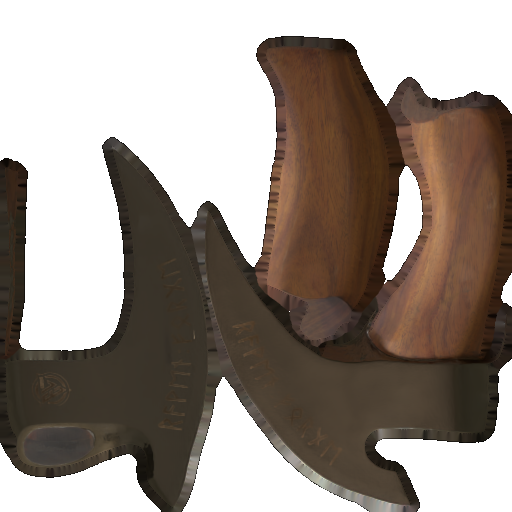
\includegraphics[width=0.47\linewidth]{assets/update_23_07/figure_1/baked_uv_texture.png} \\
        {\scriptsize Mesh} & {\scriptsize Baked Texture}
      \end{tabular}
    \end{minipage}
    &
    \begin{minipage}[c]{0.08\textwidth}
      \centering
      {\Large $\longrightarrow$}\\[0.2em]
      {\tiny\bfseries Material\\Estimation}
    \end{minipage}
    &
    % Right side: Target PBR UV maps
    \begin{minipage}[c]{0.47\textwidth}
      \centering
      \begin{tabular}{@{}c@{\hspace{0.2em}}c@{\hspace{0.2em}}c@{}}
        \multicolumn{3}{c}{\textbf{\scriptsize PBR Texture}}\\[0.2em]
        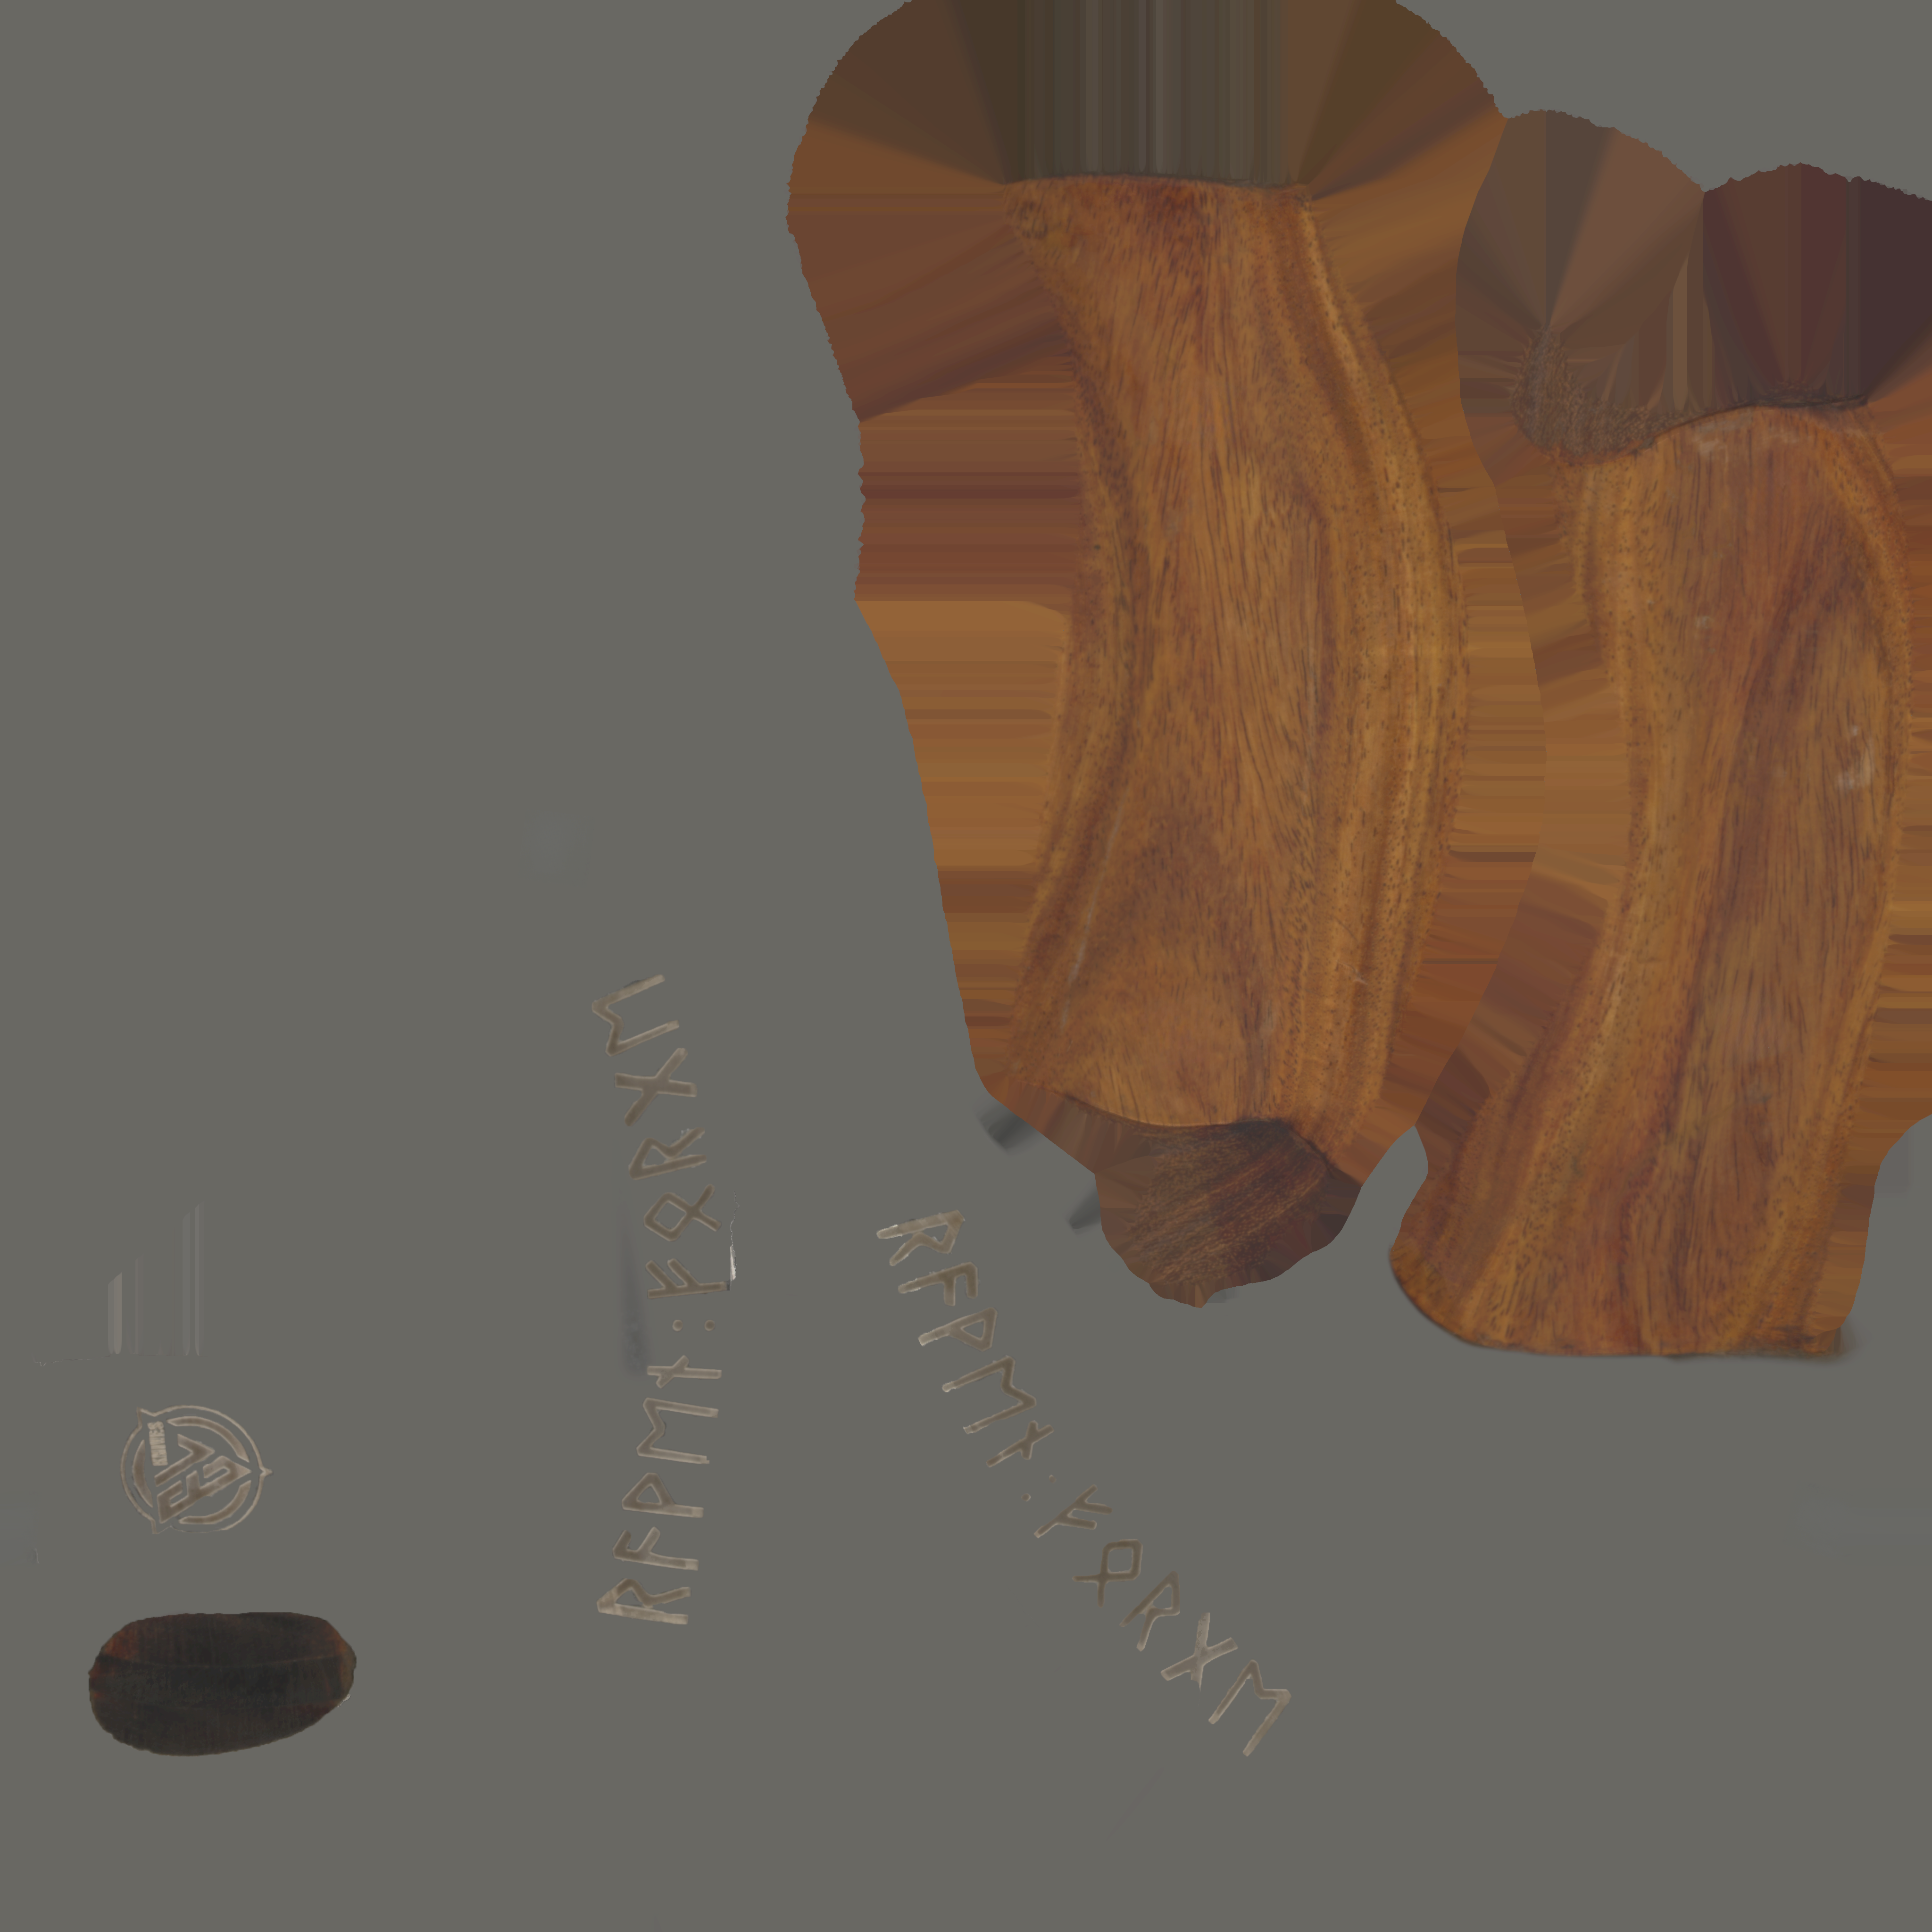
\includegraphics[width=0.31\linewidth]{assets/update_23_07/figure_1/albedo_uv.png} &
        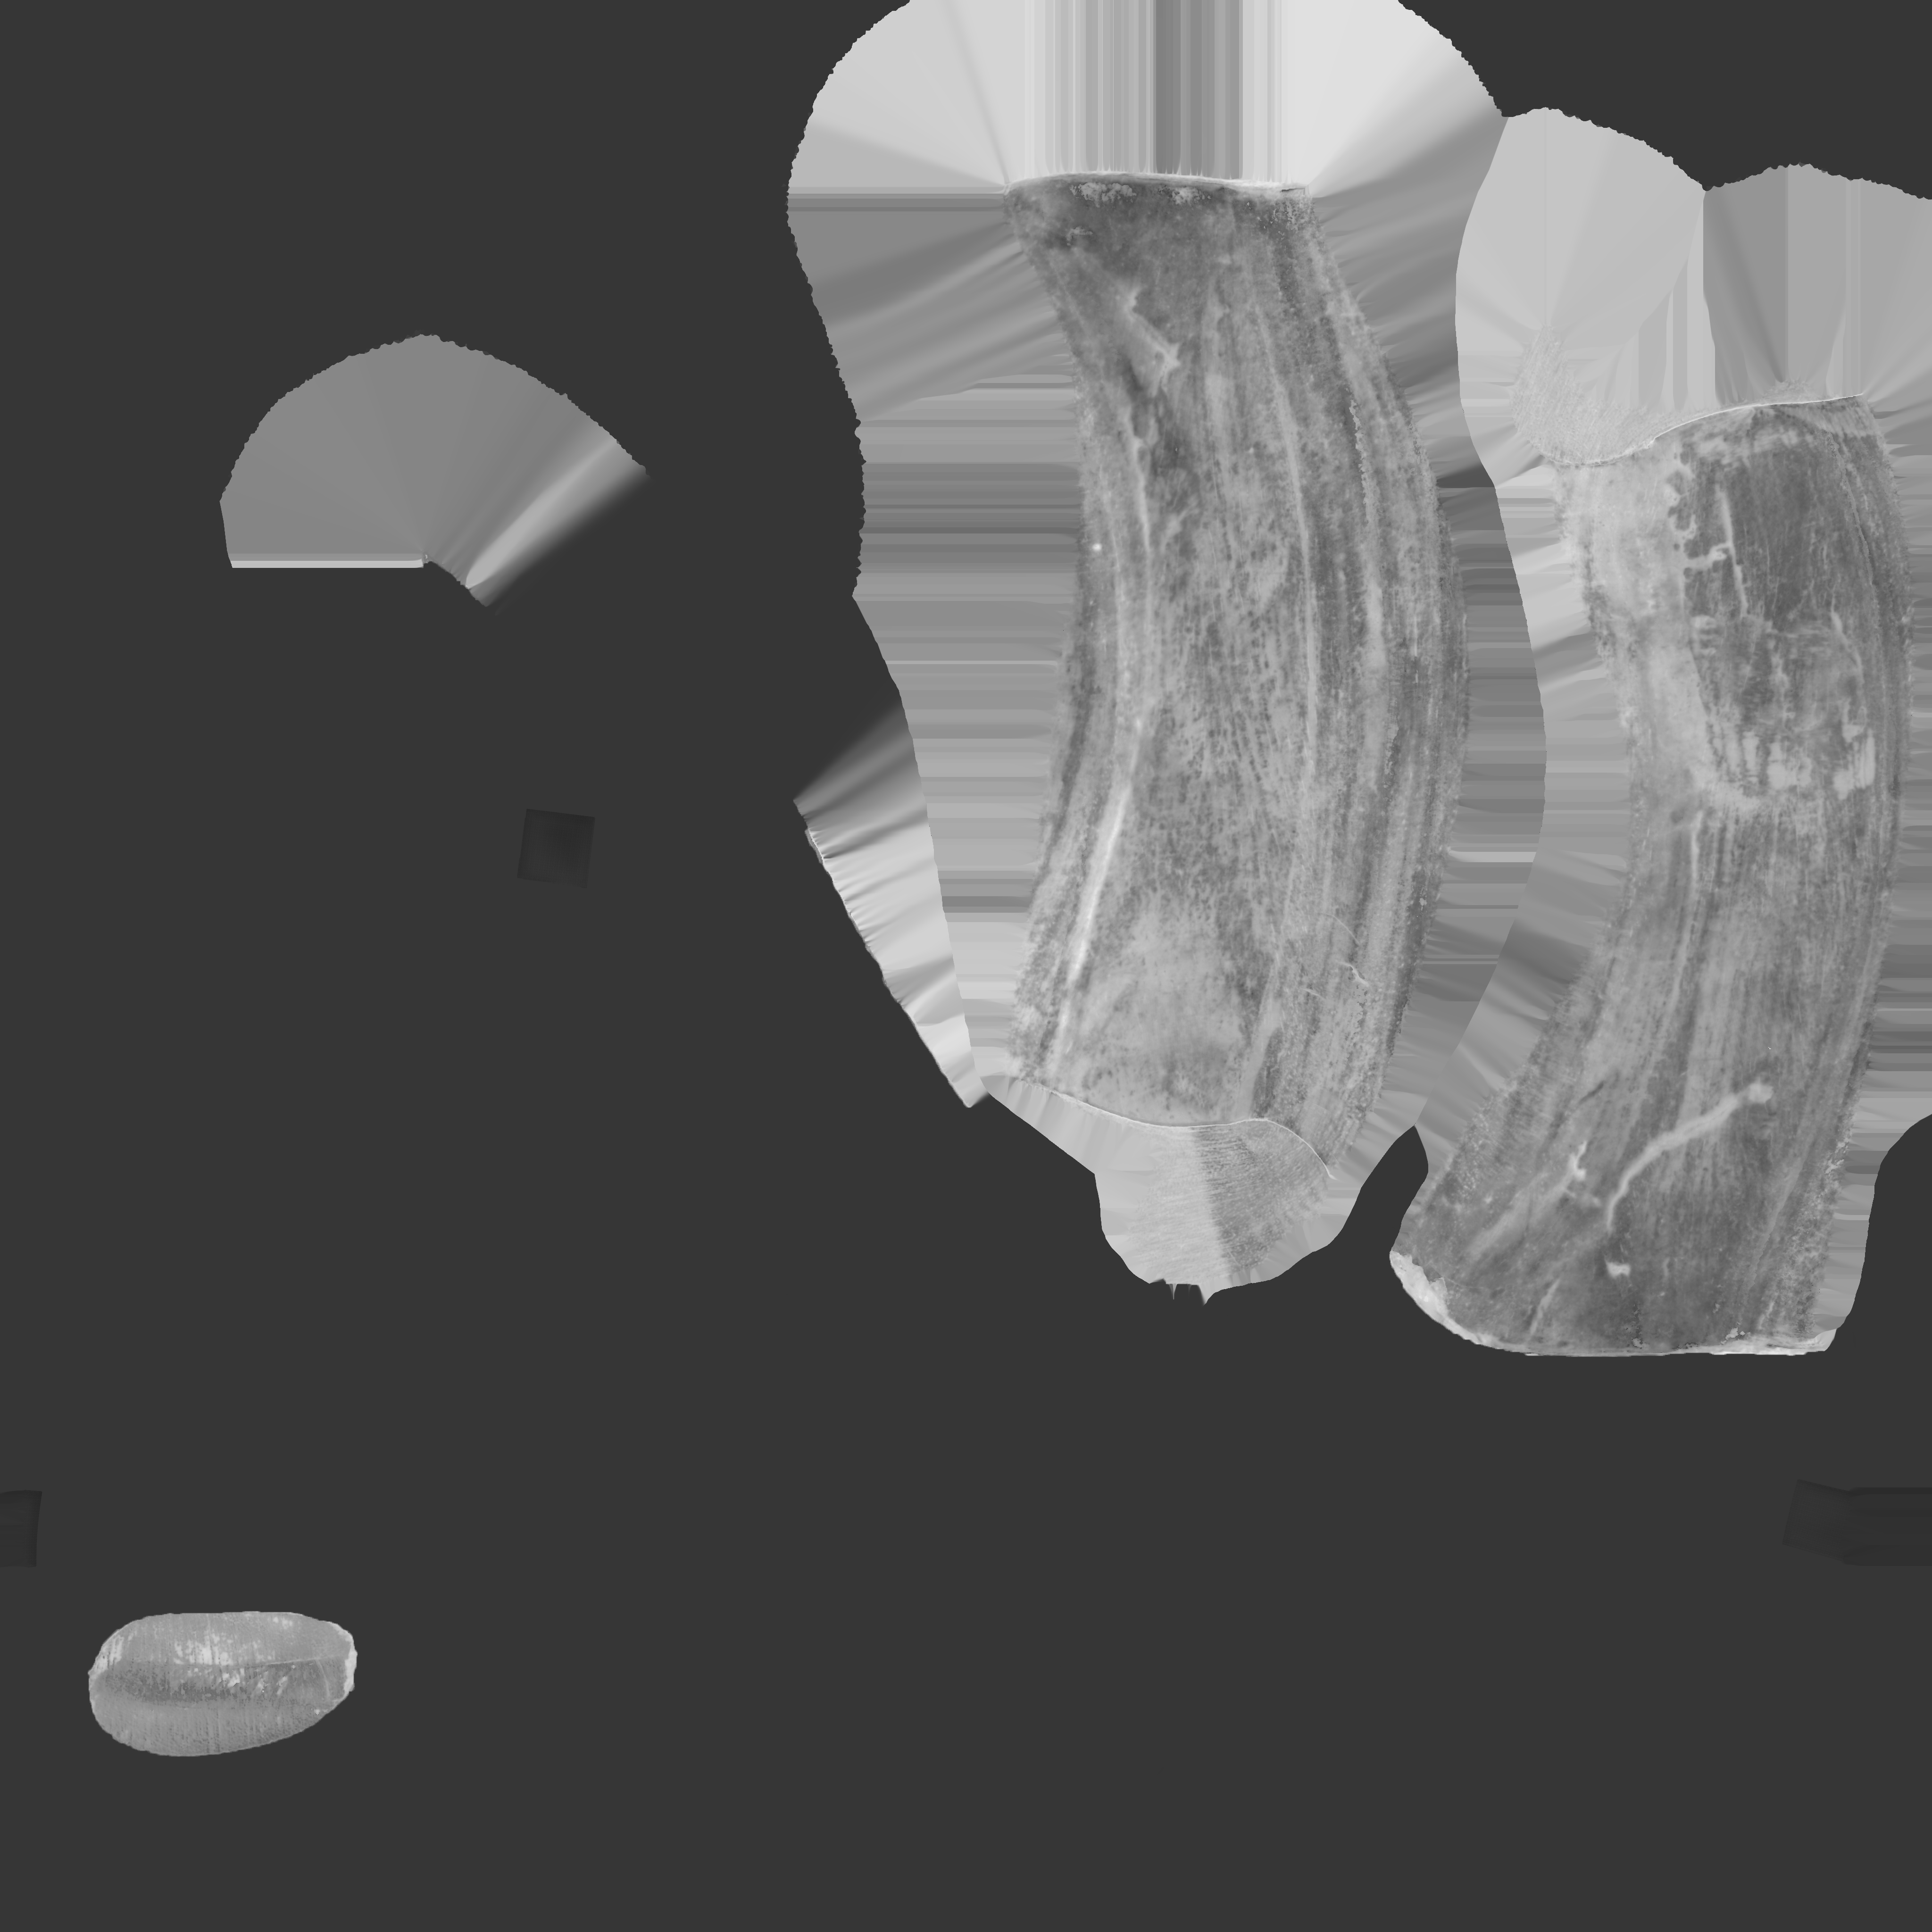
\includegraphics[width=0.31\linewidth]{assets/update_23_07/figure_1/roughness_uv.png} &
        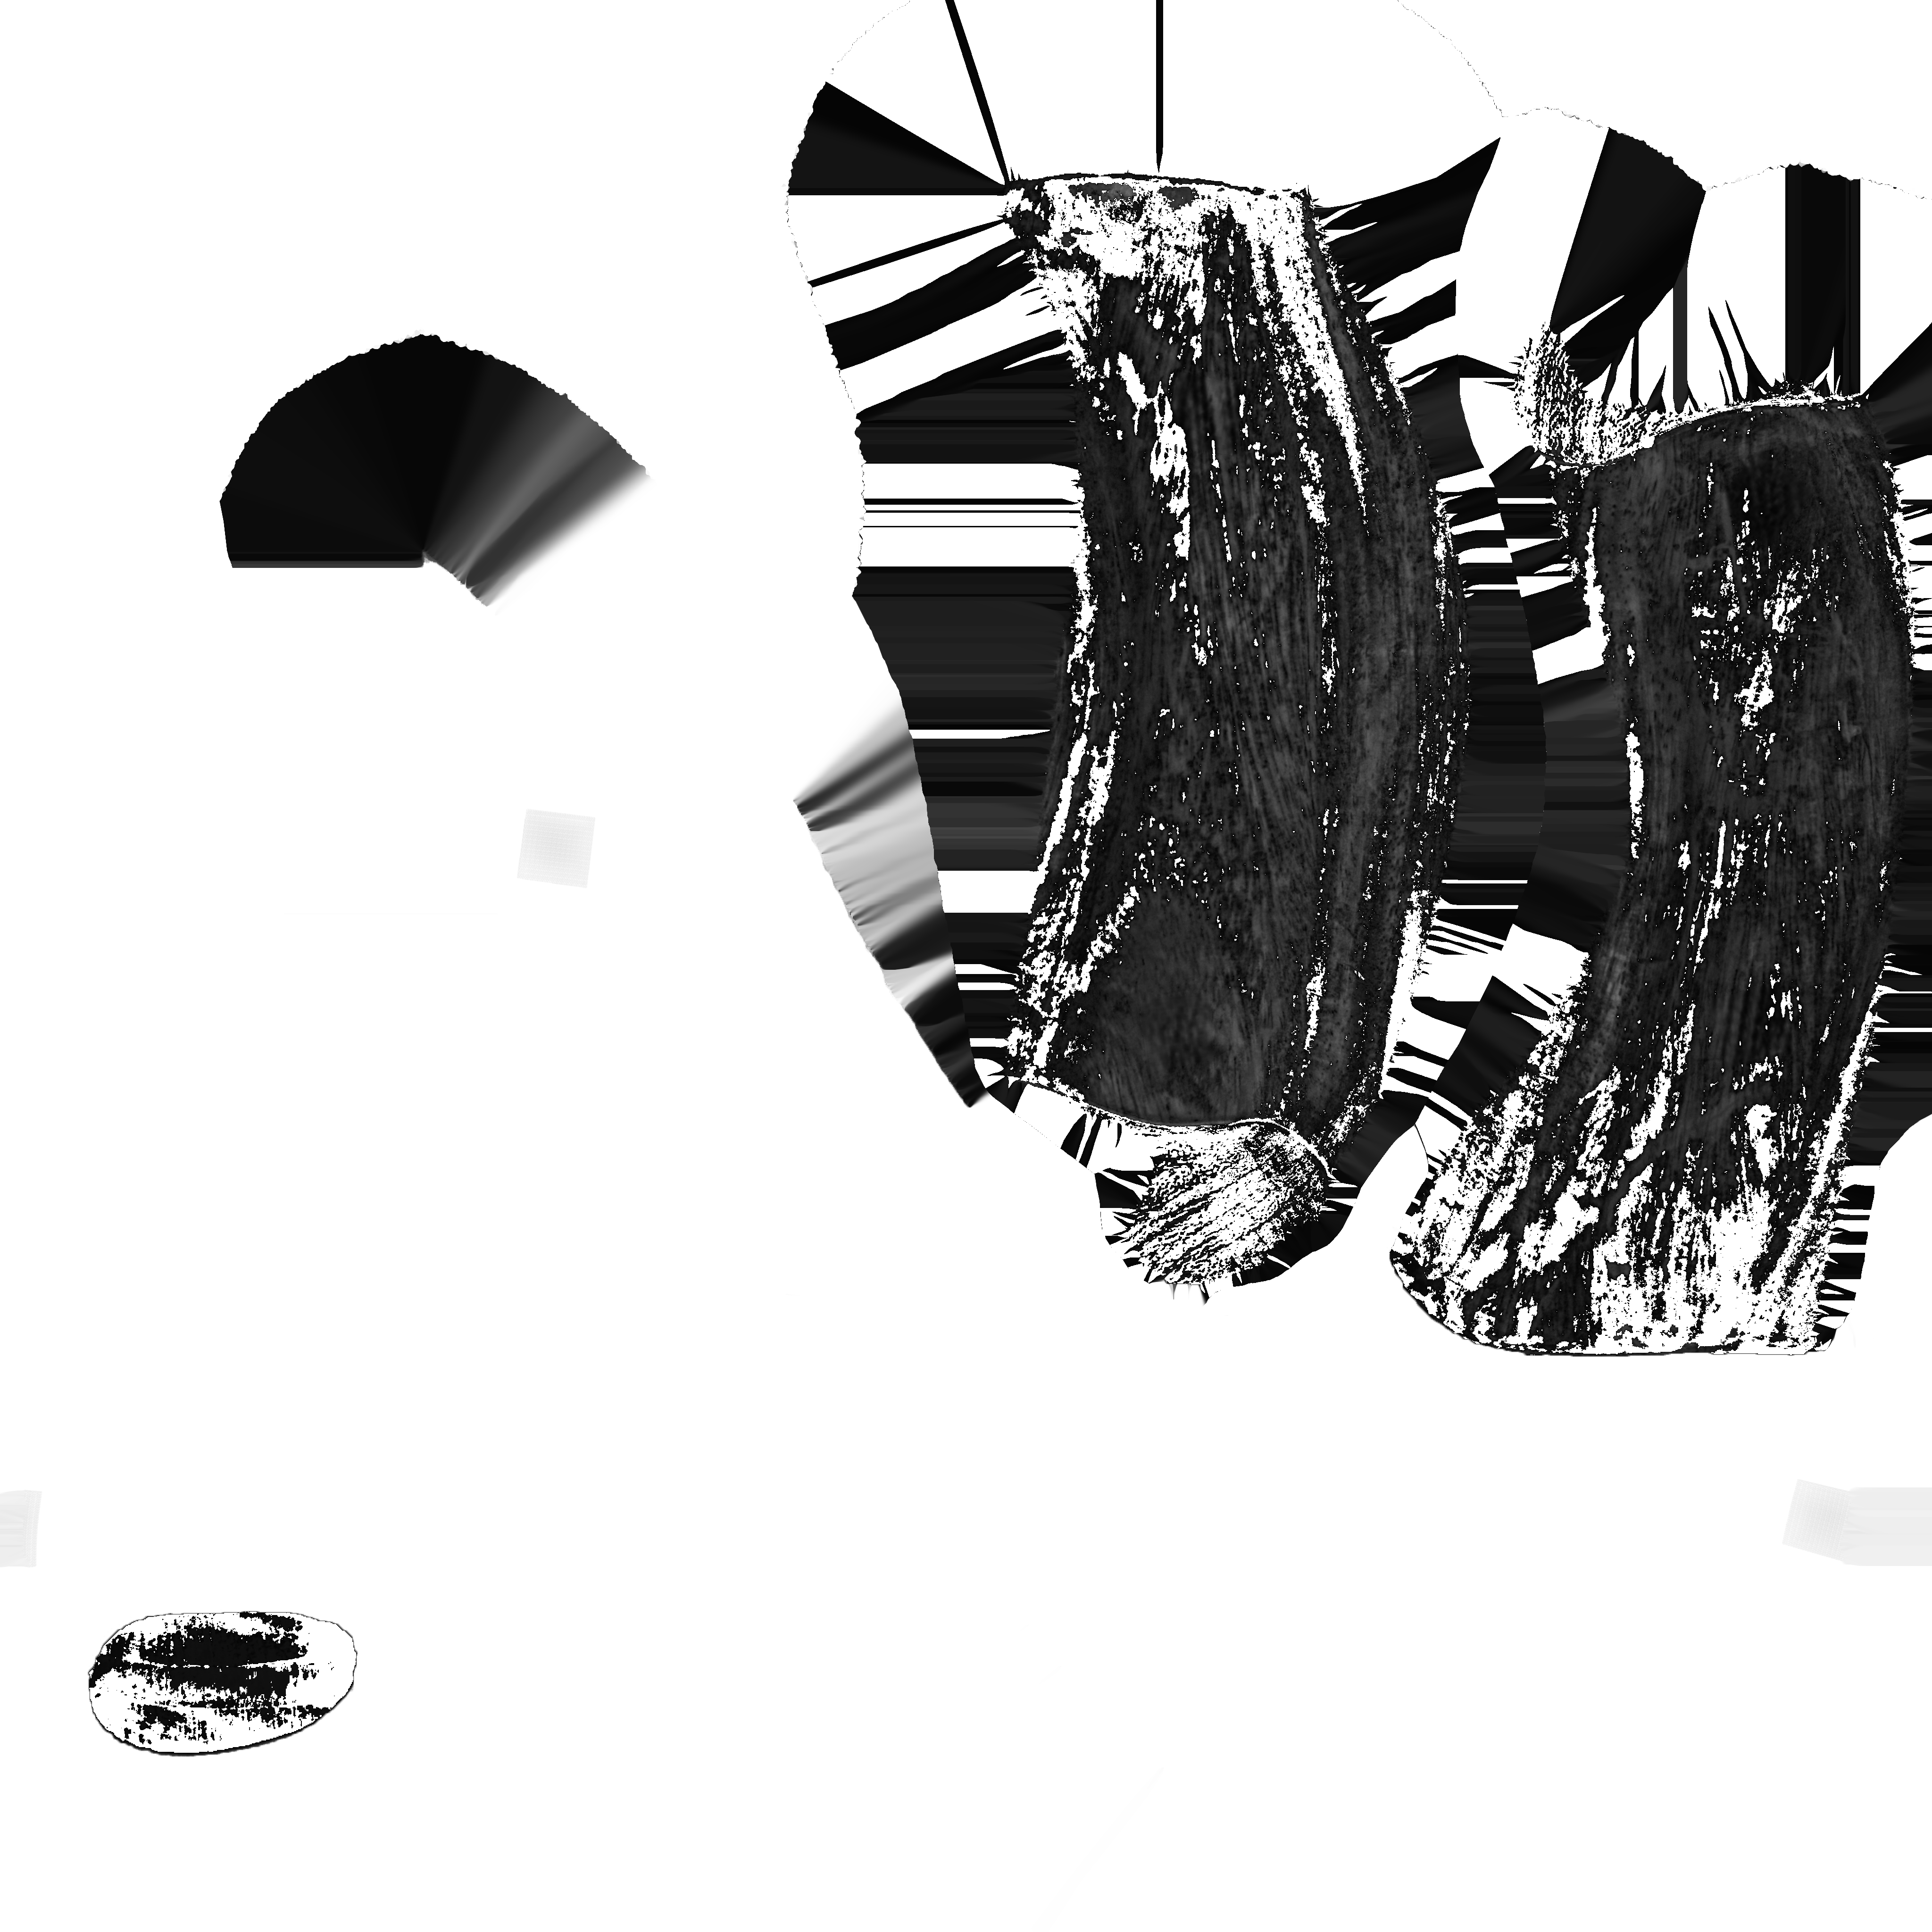
\includegraphics[width=0.31\linewidth]{assets/update_23_07/figure_1/metallic_uv.png} \\
        {\scriptsize Base Colour} & {\scriptsize Roughness} & {\scriptsize Metallic}
      \end{tabular}
    \end{minipage}
  \end{tabular}
  \caption{\textbf{Problem formulation:} Given a mesh with a texture map containing baked illumination, the goal is to estimate relightable PBR material maps (base colour, perceptual roughness, and metallic).}
  \label{fig:problem-formulation}
\end{figure}

\section{Evaluation Protocol}

There isn't an established protocol for evaluating PBR material estimation. Various methods have slightly differing problem formulations, evaluate on different datasets, and focus on different metrics. Nevertheless, most evaluations revolve around testing against synthetic data, for which ground truth PBR textures are available~\cite{neurallightrig, supermat, matmart, diffusionrenderer}. Many prior works focus on error minimization against ground truth using RMSE and PSNR on intrinsic channels and rerendered views, while others measure distributional metrics like FID or conduct user studies~\cite{materialanything}, and some rely purely on qualitative assessment~\cite{trellis2}.

To address this fragmentation and assess method robustness under changing conditions, we standardize evaluation for object-level inverse rendering.

\subsection{Direct Evaluation}

In direct evaluation, we task methods with unbaking illumination from object texture maps. Assets are sourced from four distinct datasets: Objaverse~\cite{objaverse}, Poly Haven~\cite{polyhaven}, Digital Twin Catalog (DTC)~\cite{dtc}, and TexVerse~\cite{texverse}. We curate 64 objects per dataset spanning diverse geometries and material types, rendered under 4 distinct HDRI environment maps (indoor, studio, outdoor overcast, and outdoor sunny), producing 1,024 evaluation samples per method.

We evaluate reconstruction fidelity via PSNR and RMSE across 2D projected intrinsic channels. This 2D projection allows unified comparison between 3D-native approaches and 2D single-view material estimation baselines. Additionally, across the 4 illumination conditions per object, we record prediction variance ($\sigma_{\text{light}}$) to assess illumination sensitivity and stability under varying lighting.

\subsection{Evaluation via Rerendering}

Measuring direct intrinsic channel reconstruction error only tells part of the story. Material estimation is inherently an ill-posed problem, as no unique decomposition exists for a single observation—an assumption implicitly made by direct channel metrics. Furthermore, in practice, the primary goal of material estimation is not exact pixel-level intrinsic recovery, but rather estimating material properties that behave realistically under varying lighting conditions. As such, we complement direct evaluation with indirect rerendering evaluation using Blender (EEVEE/Cycles). We evaluate relighting fidelity under novel target illumination ($\text{target\_envmap} \neq \text{input\_light}$) using standard image quality metrics (PSNR, SSIM, LPIPS) computed over masked object silhouettes. Furthermore, we single out cycle-consistency under identity illumination ($\text{target\_envmap} = \text{input\_light}$), which measures reconstruction error when rerendering an object under its original input lighting. This diagnostic is particularly valuable for examining how methods handle highly reflective objects: if a method bakes input illumination into its estimated albedo map, cycle-consistency performance can remain deceptively high while relighting fidelity under novel illumination degrades significantly.

\section{Baselines}

We evaluate three 2D single-view inverse rendering baseline methods: \textbf{SuperMat}~\cite{supermat}, \textbf{Neural LightRig}~\cite{neurallightrig}, and \textbf{DiffusionRenderer}~\cite{diffusionrenderer}. These methods estimate PBR material channels (base colour $\sigma$, roughness $\alpha$, metallic $m$) from single-view RGB imagery using fast UNet material decomposition, multi-light diffusion conditioning, or video-based neural inverse rendering priors, respectively.

\subsection{Oracle Reference Baseline: PBROracleSV (Ours)}

To establish a performance upper-bound for single-view material estimation via generative relighting, we construct an oracle baseline, \textbf{PBROracleSV (Ours)}. This baseline assumes access to an ideal generative relighting model that, given a single-view input image $I_{\text{src}}$ of a baked object, can re-illuminate it under target environment lighting $E$. Specifically, we simulate this relighting capability in Blender (Cycles) using ground-truth 3D assets to render relit views $I_{\text{relit}}$. Crucially, PBROracleSV operates \emph{only} on these relit views and never accesses the ground-truth PBR texture maps directly.

Inspired by physics-guided relighting frameworks such as SwitchLight~\cite{switchlight}, we first separate overall image formation into diffuse reflection ($I_{\text{diff}}$) and specular reflection ($I_{\text{spec}}$):
\begin{equation}
  I = I_{\text{diff}} + I_{\text{spec}}
\end{equation}
where diffuse reflection uniform scatters light following the Lambertian BRDF ($f_d = \frac{\sigma}{\pi}$). To extract the diffuse albedo $\sigma$, our pipeline proceeds in two steps:
\begin{enumerate}
  \item \textbf{Diffuse Shading Estimation:} We first render the object geometry with a unit, perfectly diffuse Lambertian material ($\sigma = 1$) under target illumination $E$, isolating the pure diffuse shading (irradiance map):
  \begin{equation}
    S_{\text{diff}}(\mathbf{n}, E) = \int_{\Omega} E(\mathbf{l}) \langle \mathbf{n} \cdot \mathbf{l} \rangle \, d\mathbf{l}
  \end{equation}
  \item \textbf{Diffuse Albedo Extraction:} Next, we obtain a relit observation of the object $I_{\text{relit}}$ under its true materials. By isolating the diffuse render $I_{\text{diff}}$, the diffuse albedo $\hat{\sigma}$ is computed directly by dividing the diffuse render by its diffuse shading:
  \begin{equation}
    \hat{\sigma} = \pi \cdot \frac{I_{\text{diff}}}{S_{\text{diff}}(\mathbf{n}, E)}
  \end{equation}
\end{enumerate}

We treat this extracted diffuse albedo $\hat{\sigma}$ directly as our estimated base colour. While one could extend this formulation by performing an inverse differentiable rendering optimization loop to recover non-Lambertian specular properties (roughness $\alpha$ and metallic $m$), we leave specular channel optimization for future work and focus here on single-view albedo estimation.

\subsection{Quantitative Results}

Table~\ref{tab:direct-results} reports direct material estimation performance across intrinsic channels. Table~\ref{tab:relighting-results} reports indirect relighting fidelity and cycle-consistency.

\begin{table}[htbp]
  \centering
  \small
  \setlength{\tabcolsep}{4pt}
  \resizebox{\textwidth}{!}{%
  \begin{tabular}{llccccccccc}
    \toprule
    & & \multicolumn{3}{c}{Albedo} & \multicolumn{3}{c}{Roughness} & \multicolumn{3}{c}{Metallic}\\
    \cmidrule(lr){3-5}\cmidrule(lr){6-8}\cmidrule(lr){9-11}
    Dataset & Method & PSNR$\uparrow$ & RMSE$\downarrow$ & $\sigma_{\text{light}}\downarrow$ & PSNR$\uparrow$ & RMSE$\downarrow$ & $\sigma_{\text{light}}\downarrow$ & PSNR$\uparrow$ & RMSE$\downarrow$ & $\sigma_{\text{light}}\downarrow$\\
    \midrule
    \multirow{4}{*}{DTC}
     & SuperMat           & 19.73 & 0.136 & 0.056 & 18.82 & 0.134 & 0.067 & 22.09 & 0.158 & 0.101 \\
     & DiffusionRenderer  & 13.92 & 0.247 & 0.096 & 13.01 & 0.286 & 0.107 & 21.62 & 0.237 & 0.116 \\
     & Neural LightRig    & 19.17 & 0.137 & 0.060 & 14.14 & 0.222 & 0.102 & 18.32 & 0.205 & 0.124 \\
     & PBROracleSV (Ours) & 28.67 & 0.043 & 0.000 & -- & -- & -- & -- & -- & -- \\
    \midrule
    \multirow{4}{*}{Objaverse}
     & SuperMat           & 20.08 & 0.133 & 0.047 & 14.57 & 0.220 & 0.074 & 16.64 & 0.236 & 0.099 \\
     & DiffusionRenderer  & 15.20 & 0.220 & 0.085 & 13.28 & 0.271 & 0.090 & 18.65 & 0.290 & 0.076 \\
     & Neural LightRig    & 18.47 & 0.151 & 0.055 & 13.68 & 0.238 & 0.100 & 15.02 & 0.261 & 0.117 \\
     & PBROracleSV (Ours) & 26.53 & 0.069 & 0.000 & -- & -- & -- & -- & -- & -- \\
    \midrule
    \multirow{4}{*}{Poly Haven}
     & SuperMat           & 20.98 & 0.110 & 0.044 & 16.40 & 0.169 & 0.072 & 17.44 & 0.214 & 0.115 \\
     & DiffusionRenderer  & 15.11 & 0.216 & 0.075 & 12.08 & 0.291 & 0.097 & 16.79 & 0.313 & 0.104 \\
     & Neural LightRig    & 19.66 & 0.125 & 0.049 & 13.64 & 0.234 & 0.089 & 12.72 & 0.309 & 0.142 \\
     & PBROracleSV (Ours) & 26.37 & 0.068 & 0.000 & -- & -- & -- & -- & -- & -- \\
    \midrule
    \multirow{4}{*}{TexVerse}
     & SuperMat           & 18.69 & 0.151 & 0.042 & 14.50 & 0.218 & 0.064 & 13.57 & 0.306 & 0.114 \\
     & DiffusionRenderer  & 14.18 & 0.235 & 0.087 & 11.74 & 0.301 & 0.069 & 11.70 & 0.415 & 0.113 \\
     & Neural LightRig    & 18.32 & 0.162 & 0.047 & 14.11 & 0.225 & 0.091 & 11.37 & 0.341 & 0.144 \\
     & PBROracleSV (Ours) & 24.30 & 0.101 & 0.000 & -- & -- & -- & -- & -- & -- \\
    \bottomrule
  \end{tabular}%
  }
  \caption{Direct PBR material map estimation accuracy and light-induced variance ($\sigma_{\text{light}}$) across benchmark splits (64 objects, 1,024 evaluations per method).}
  \label{tab:direct-results}
\end{table}

\begin{table}[htbp]
  \centering
  \small
  \setlength{\tabcolsep}{4pt}
  \resizebox{\textwidth}{!}{%
  \begin{tabular}{llcccccc}
    \toprule
    & & \multicolumn{3}{c}{Relighting (Novel Illumination)} & \multicolumn{3}{c}{Cycle-Consistency (Same Illumination)}\\
    \cmidrule(lr){3-5}\cmidrule(lr){6-8}
    Dataset & Method & PSNR$\uparrow$ & SSIM$\uparrow$ & LPIPS$\downarrow$ & PSNR$\uparrow$ & SSIM$\uparrow$ & LPIPS$\downarrow$\\
    \midrule
    \multirow{3}{*}{DTC}
     & SuperMat           & 19.94 & 0.853 & 0.102 & 20.32 & 0.862 & 0.090 \\
     & DiffusionRenderer  & 16.47 & 0.766 & 0.142 & 16.68 & 0.778 & 0.132 \\
     & Neural LightRig    & 19.37 & 0.854 & 0.098 & 20.16 & 0.879 & 0.076 \\
    \midrule
    \multirow{3}{*}{Objaverse}
     & SuperMat           & 19.99 & 0.791 & 0.130 & 20.23 & 0.800 & 0.118 \\
     & DiffusionRenderer  & 16.82 & 0.710 & 0.161 & 16.97 & 0.721 & 0.152 \\
     & Neural LightRig    & 18.69 & 0.770 & 0.134 & 19.31 & 0.794 & 0.113 \\
    \midrule
    \multirow{3}{*}{Poly Haven}
     & SuperMat           & 20.85 & 0.817 & 0.118 & 21.14 & 0.827 & 0.106 \\
     & DiffusionRenderer  & 17.19 & 0.719 & 0.161 & 17.25 & 0.730 & 0.152 \\
     & Neural LightRig    & 19.60 & 0.797 & 0.125 & 20.40 & 0.827 & 0.100 \\
    \midrule
    \multirow{3}{*}{TexVerse}
     & SuperMat           & 19.53 & 0.774 & 0.119 & 19.81 & 0.786 & 0.108 \\
     & DiffusionRenderer  & 16.29 & 0.677 & 0.165 & 16.31 & 0.687 & 0.158 \\
     & Neural LightRig    & 18.96 & 0.763 & 0.128 & 19.86 & 0.796 & 0.107 \\
    \bottomrule
  \end{tabular}%
  }
  \caption{Indirect evaluation comparing novel illumination relighting fidelity against cycle-consistency under identical input illumination.}
  \label{tab:relighting-results}
\end{table}

\clearpage

\subsection{Qualitative Results}

We present qualitative comparison grids structured across three multi-method performance tiers based on aggregate benchmark error: \textbf{Easy} (top-performing assets), \textbf{Medium} (representative assets near the benchmark median), and \textbf{Hard / Failure} (challenging assets with complex geometry or strong baked directional shadows). For each performance tier, we report both direct intrinsic material map predictions (Albedo, Roughness, Metallic) and indirect relighting rerenders under novel target illumination:
\begin{itemize}
  \item \textbf{Easy Tier} (Figures~\ref{fig:visuals-intrinsics-easy} \& \ref{fig:visuals-rerendering-easy}): Direct material predictions and novel illumination rerenders for high-performing assets.
  \item \textbf{Medium Tier} (Figures~\ref{fig:visuals-intrinsics-medium} \& \ref{fig:visuals-rerendering-medium}): Material estimations and novel illumination rerenders for representative median assets.
  \item \textbf{Hard Tier} (Figures~\ref{fig:visuals-intrinsics-hard} \& \ref{fig:visuals-rerendering-hard}): Estimations and novel illumination rerenders for challenging failure cases.
\end{itemize}

\begin{figure}[p]
  \centering
  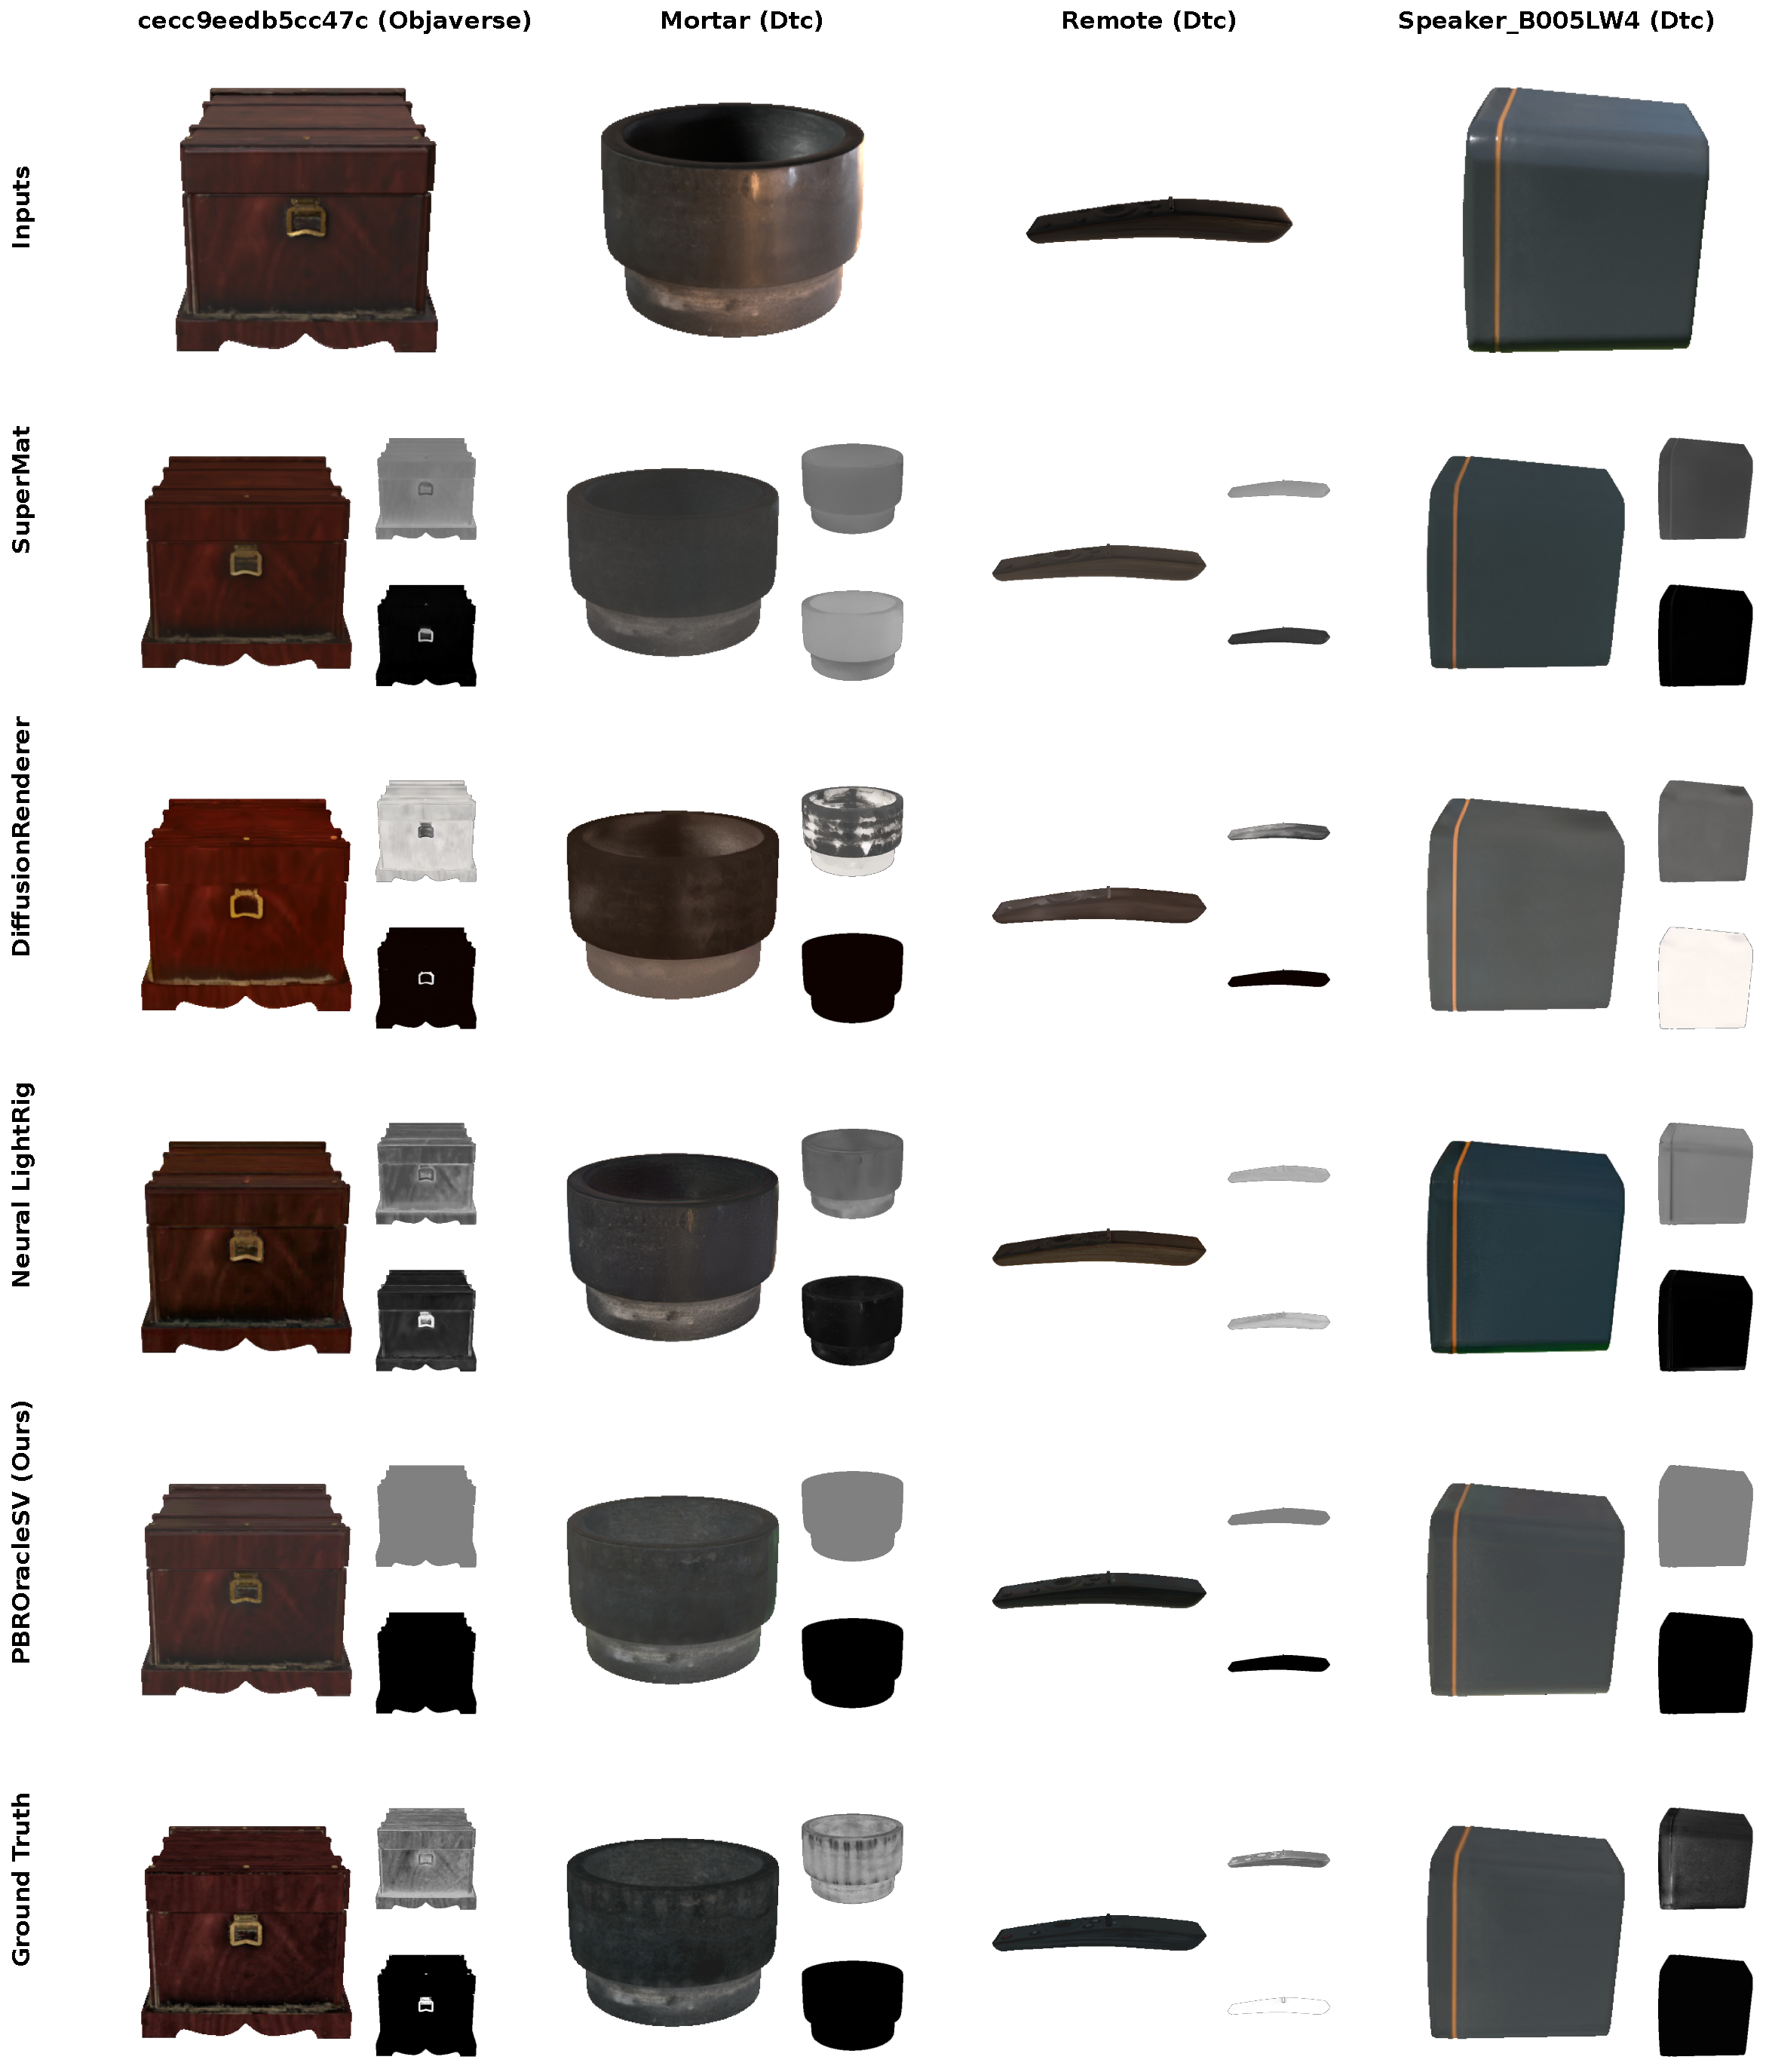
\includegraphics[width=\linewidth]{assets/update_23_07/visuals_intrinsics_easy.pdf}
  \caption{\textbf{Direct PBR material map estimation — Easy Split.} Comparison of estimated Albedo alongside Roughness and Metallic maps across 4 distinct high-performing assets.}
  \label{fig:visuals-intrinsics-easy}
\end{figure}

\begin{figure}[p]
  \centering
  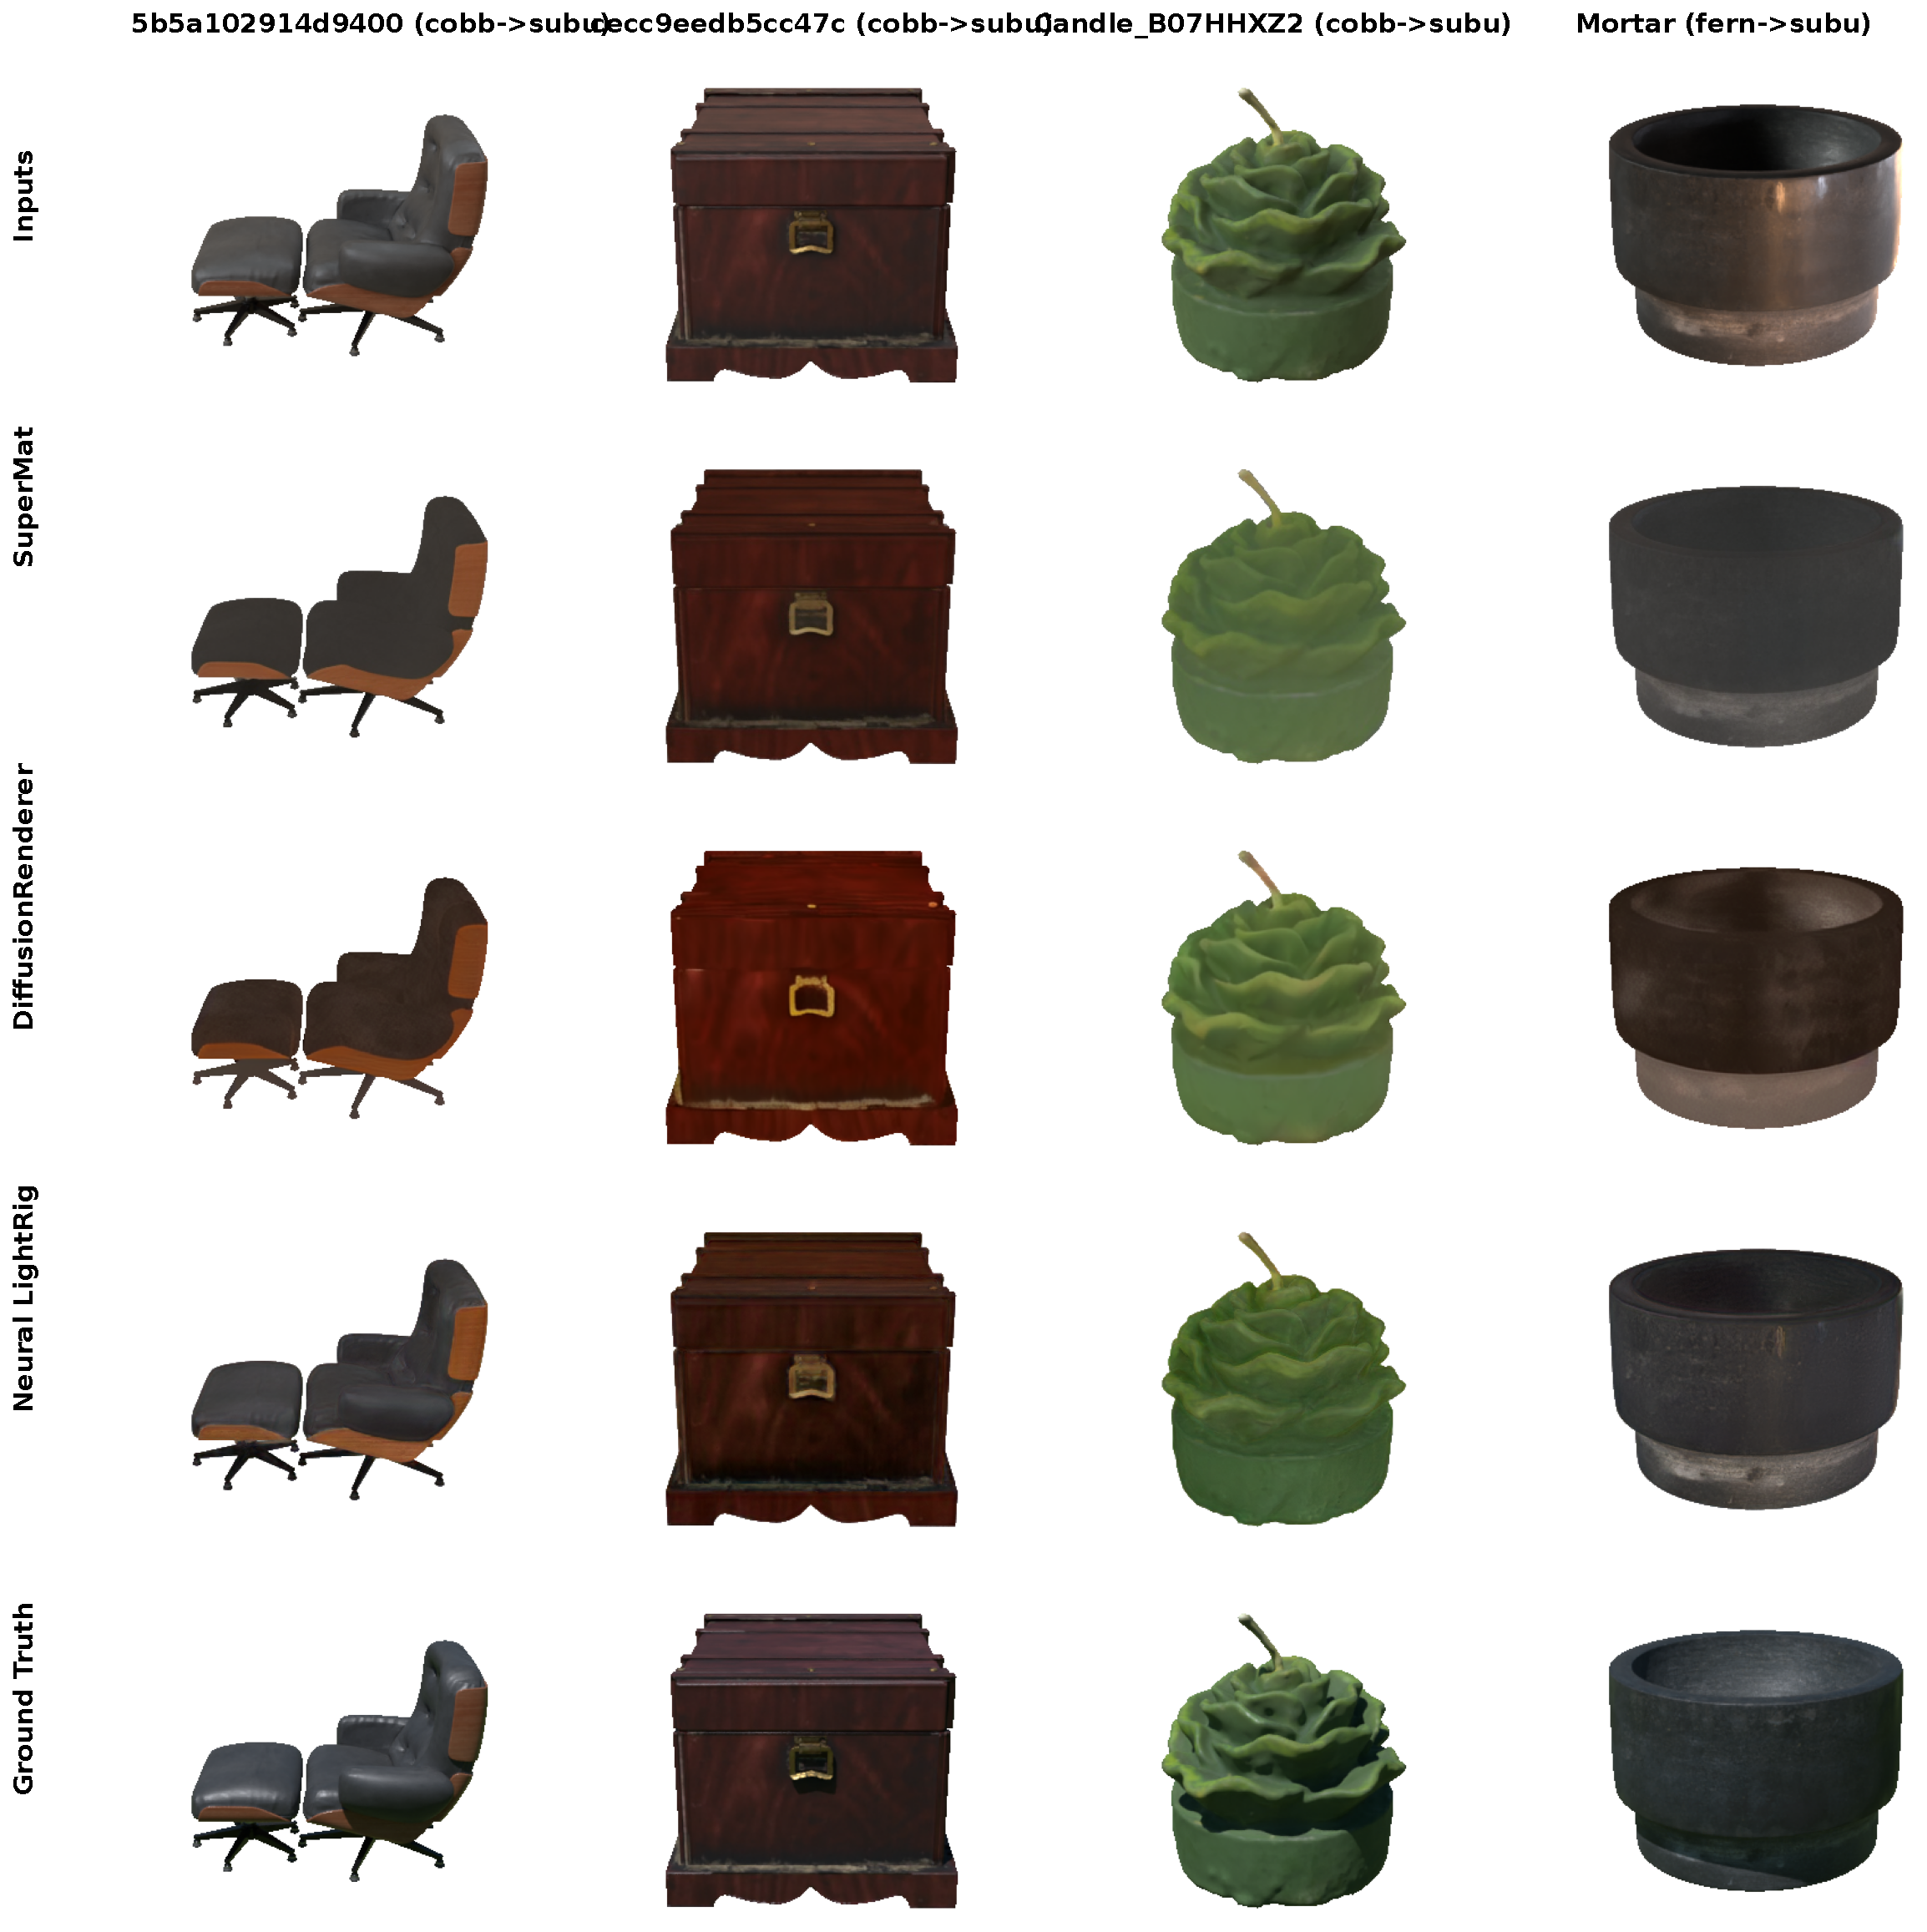
\includegraphics[width=\linewidth]{assets/update_23_07/visuals_rerendering_easy.pdf}
  \caption{\textbf{Indirect relighting evaluation — Easy Split.} Novel illumination rerenders for the distinct high-performing assets shown in Figure~\ref{fig:visuals-intrinsics-easy}.}
  \label{fig:visuals-rerendering-easy}
\end{figure}

\begin{figure}[p]
  \centering
  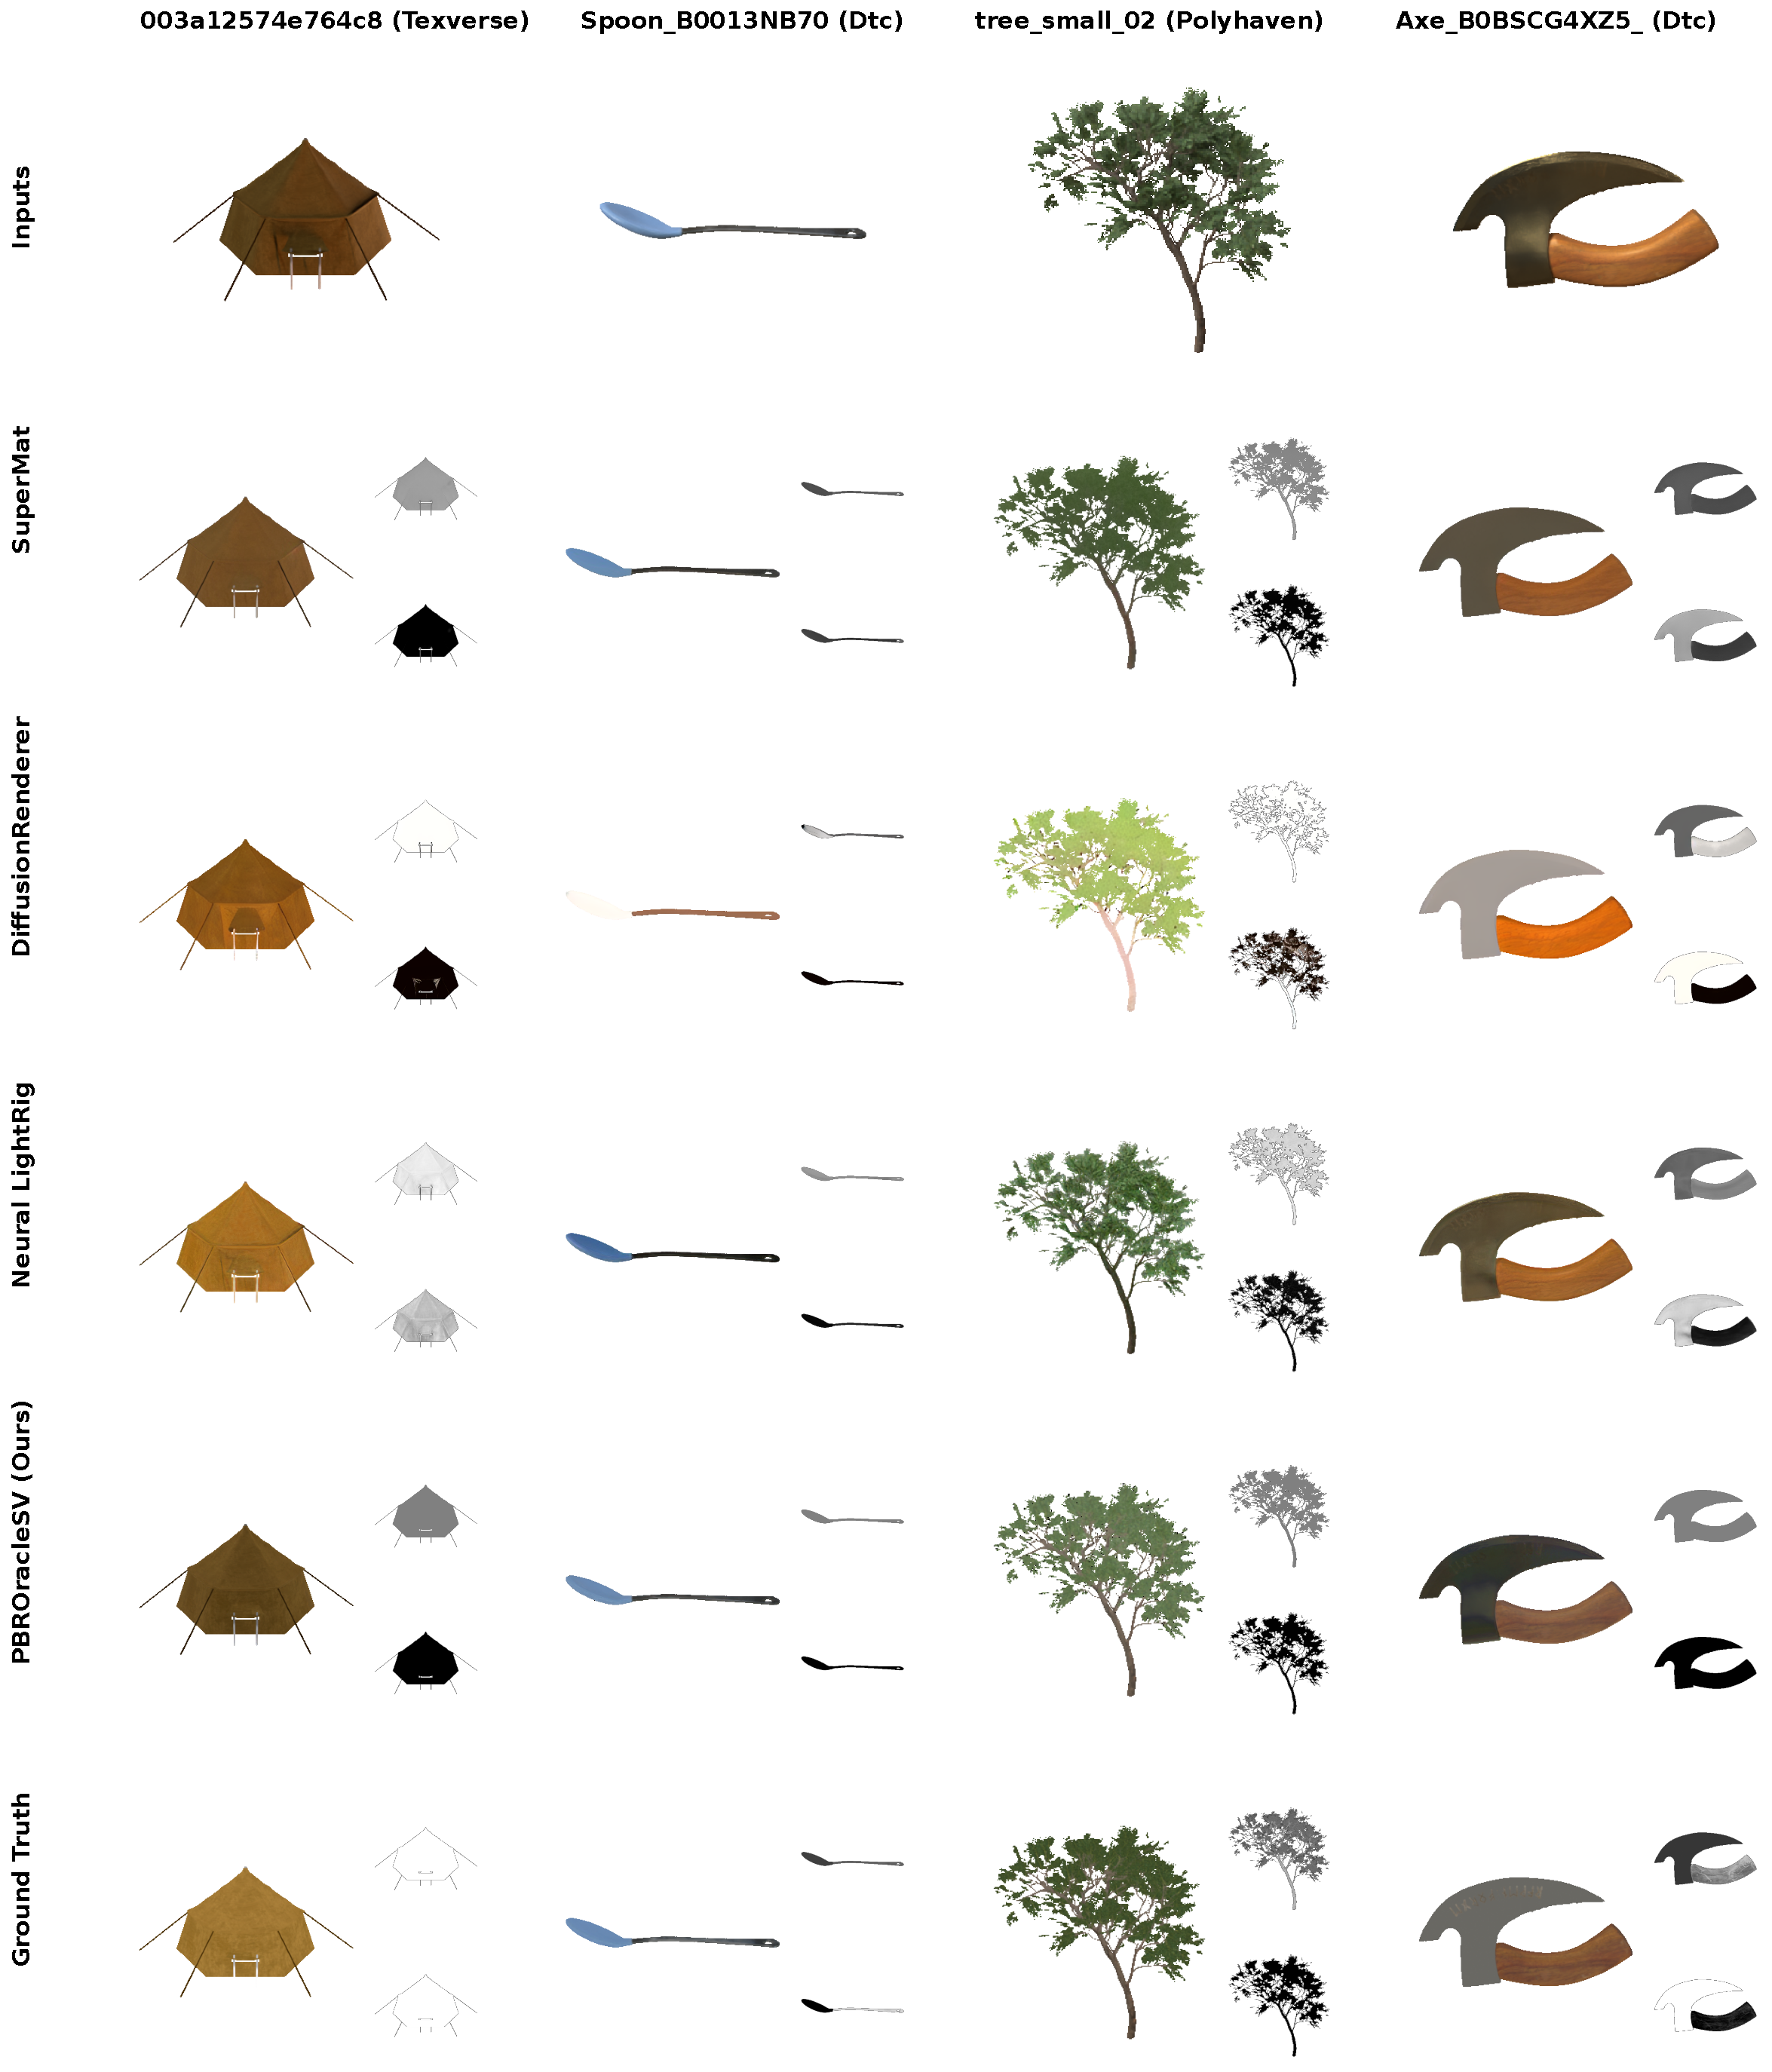
\includegraphics[width=\linewidth]{assets/update_23_07/visuals_intrinsics_medium.pdf}
  \caption{\textbf{Direct PBR material map estimation — Medium / Representative Split.} Material map predictions on 4 distinct representative assets near the benchmark median.}
  \label{fig:visuals-intrinsics-medium}
\end{figure}

\begin{figure}[p]
  \centering
  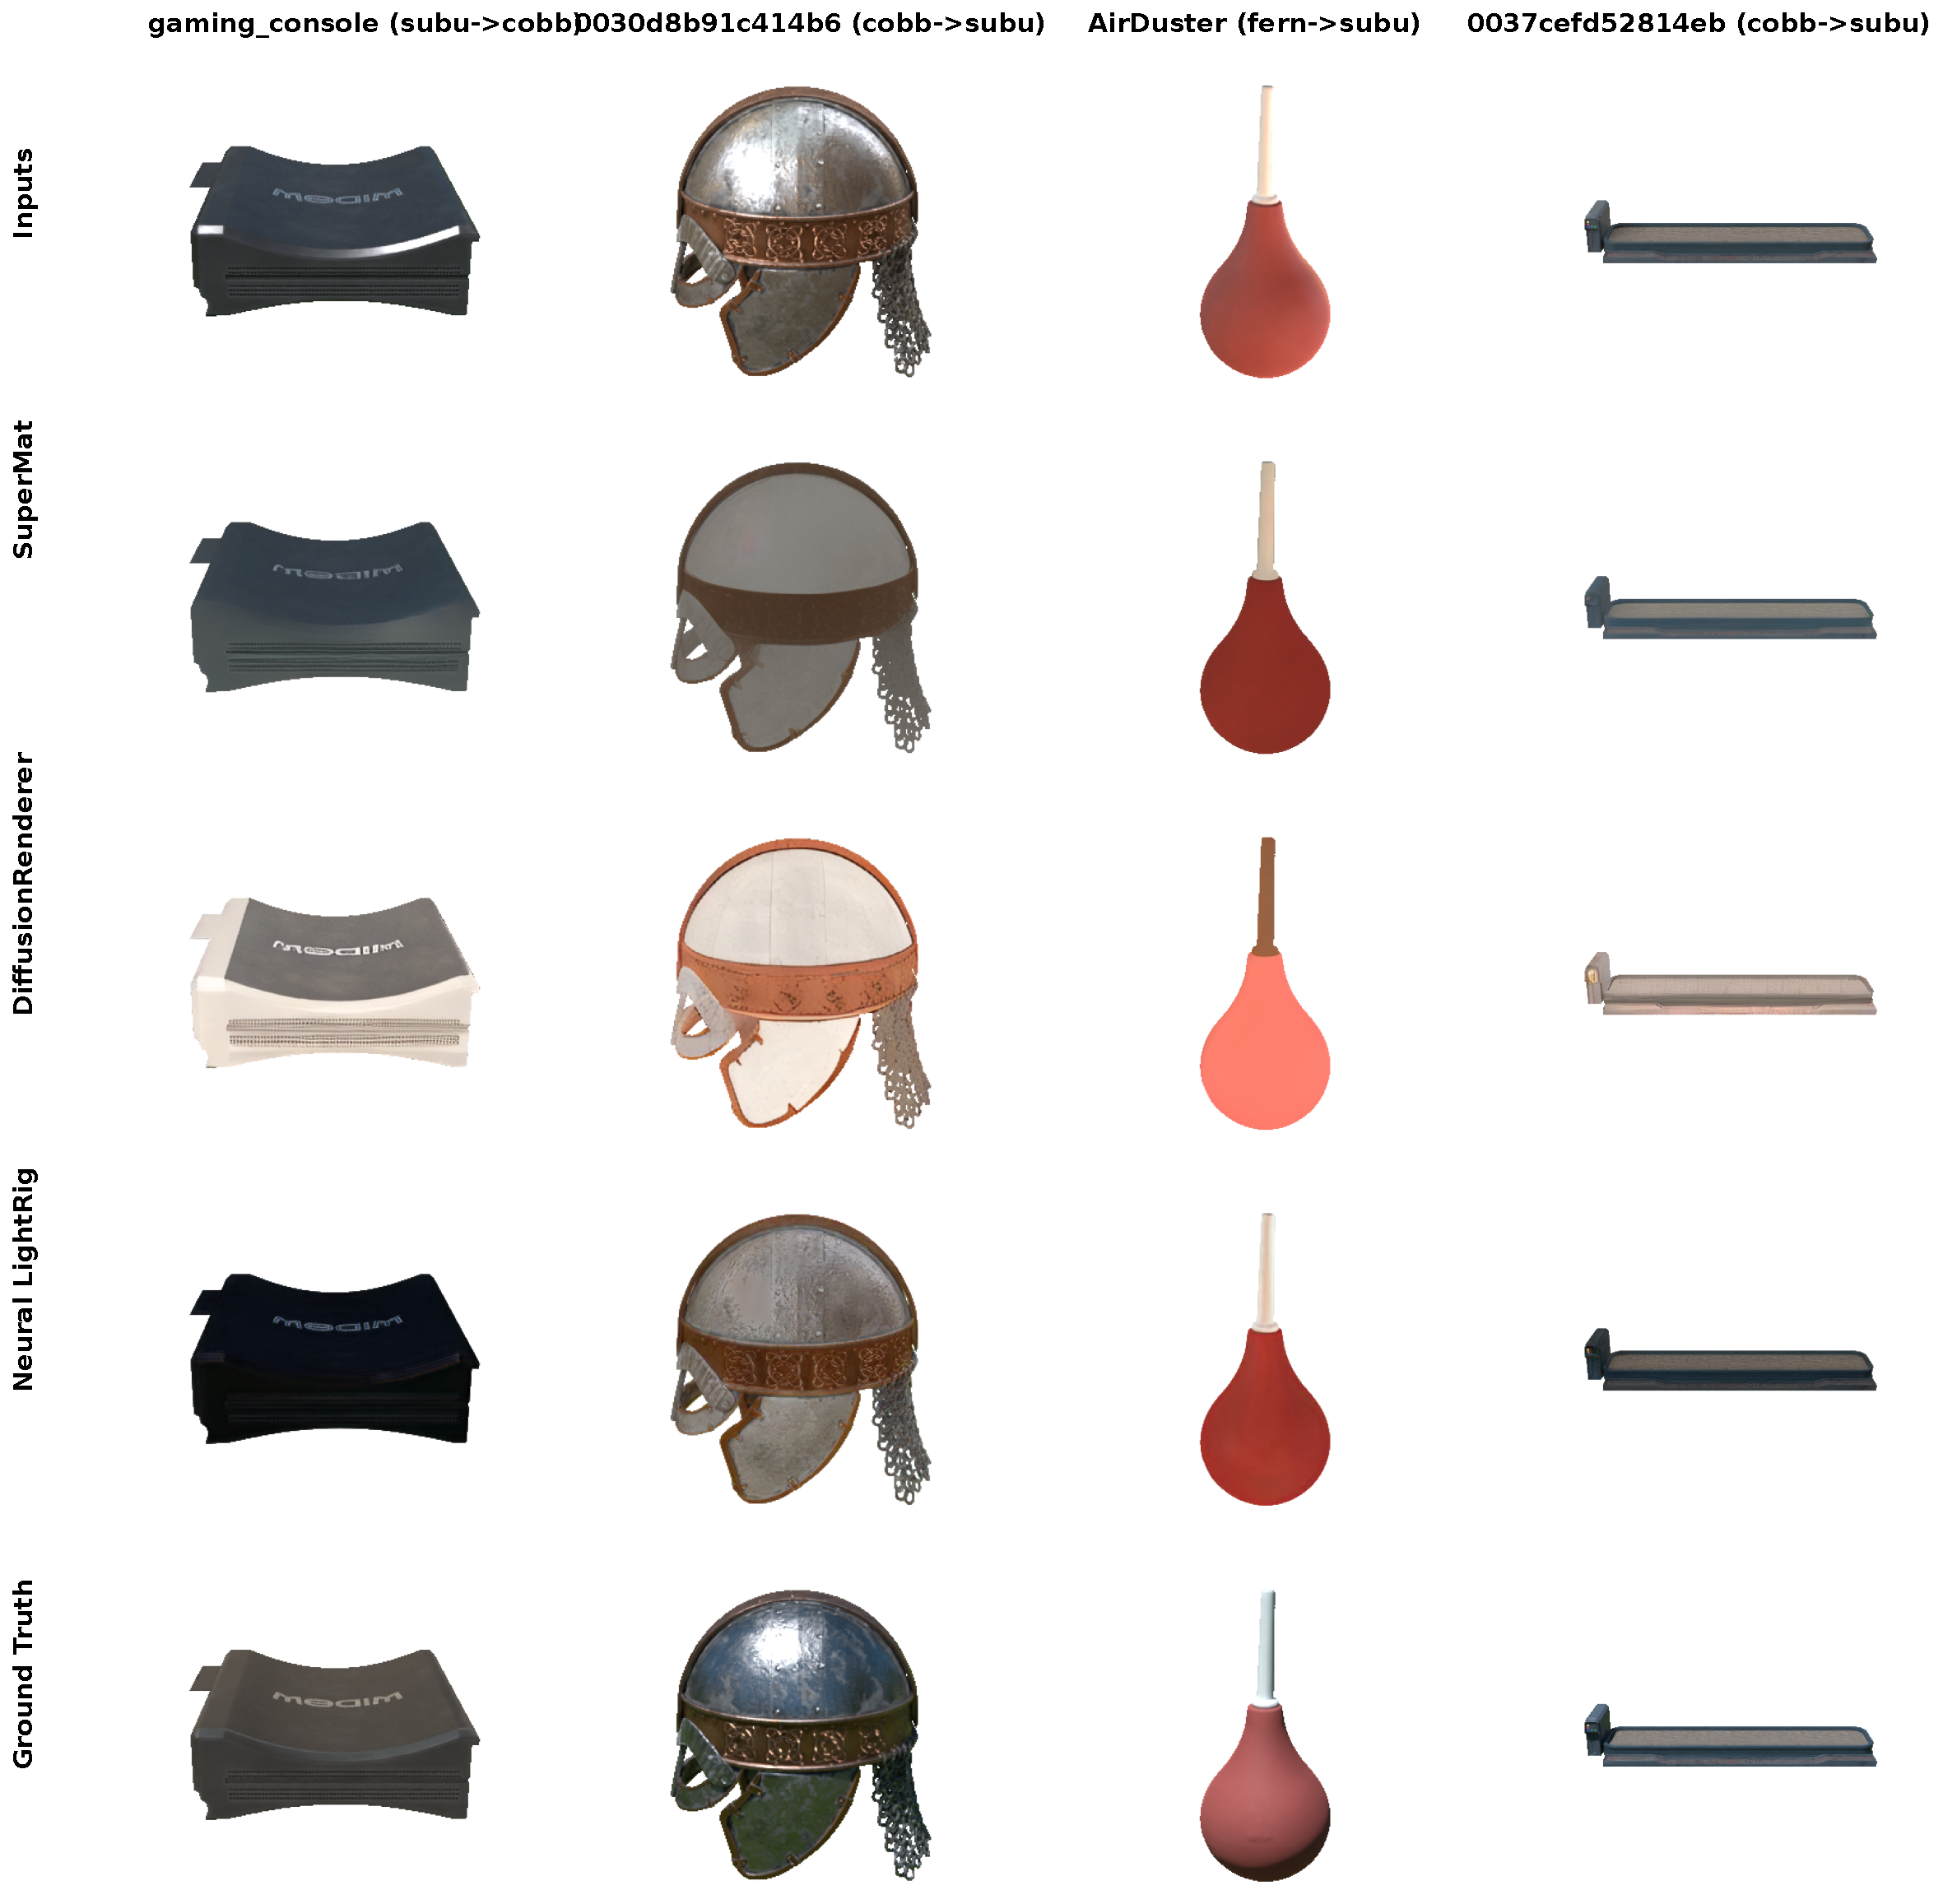
\includegraphics[width=\linewidth]{assets/update_23_07/visuals_rerendering_medium.pdf}
  \caption{\textbf{Indirect relighting evaluation — Medium / Representative Split.} Rerendered outputs under novel illumination for representative assets near the benchmark median.}
  \label{fig:visuals-rerendering-medium}
\end{figure}

\begin{figure}[p]
  \centering
  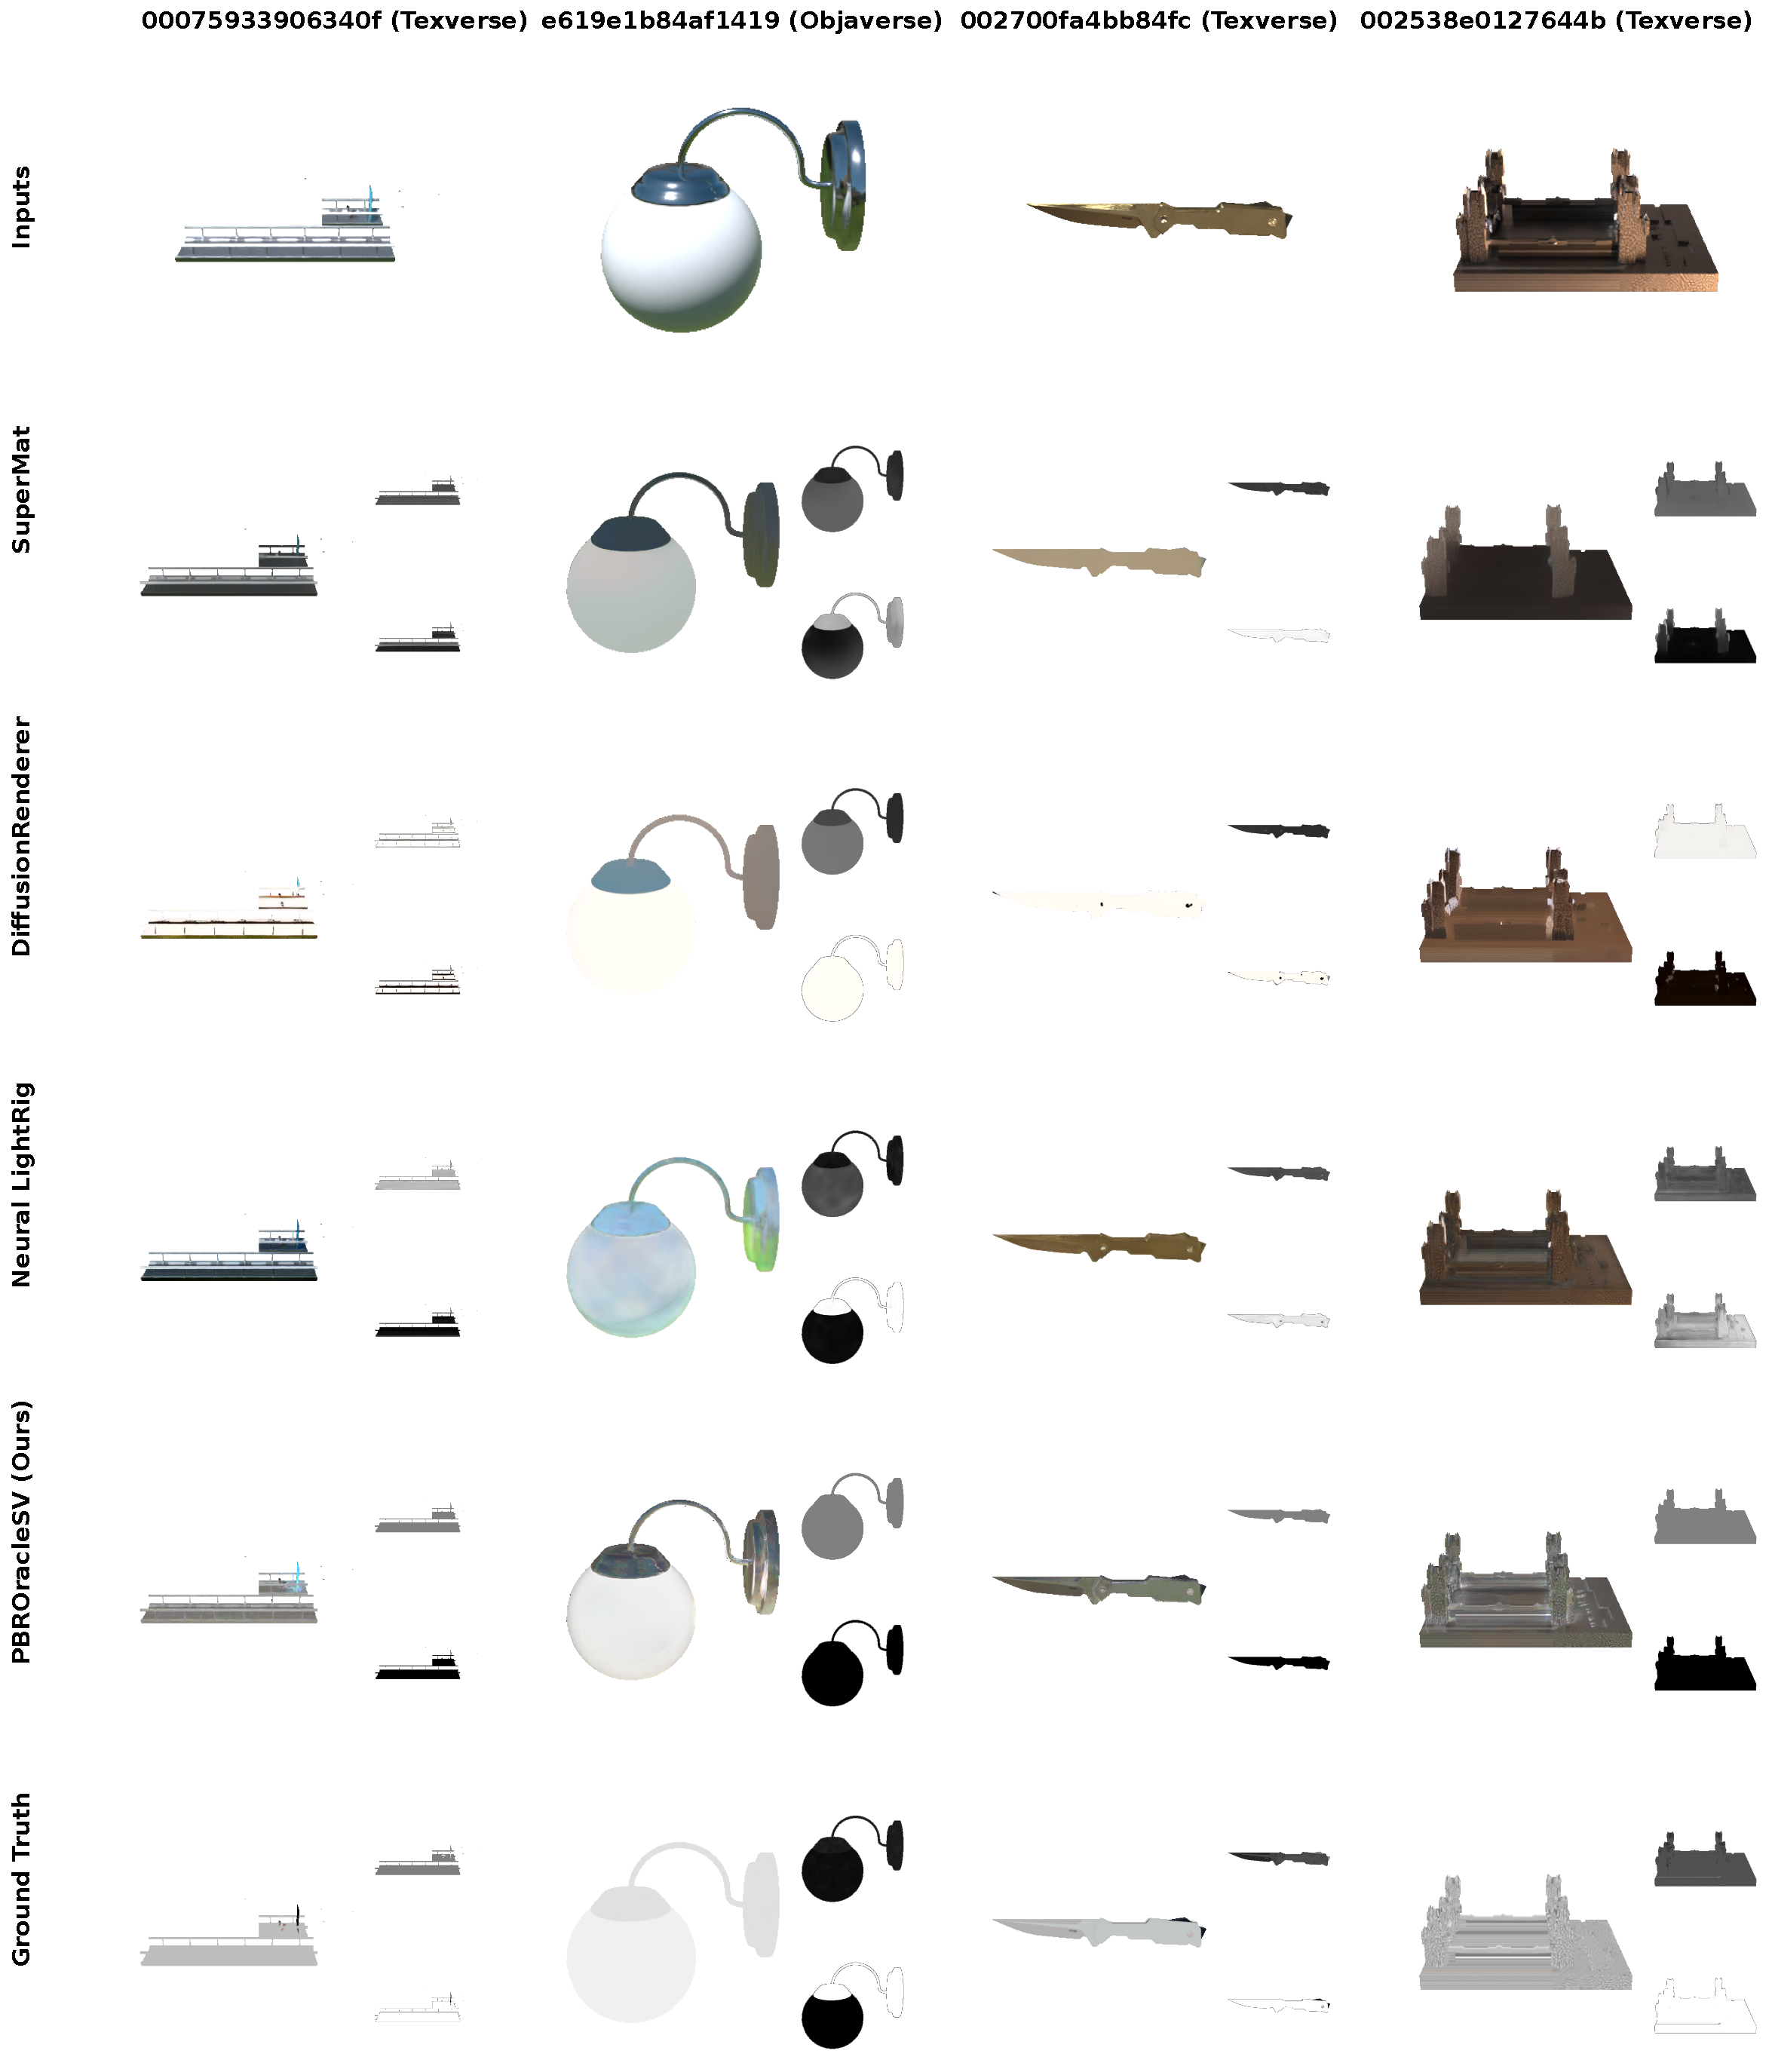
\includegraphics[width=\linewidth]{assets/update_23_07/visuals_intrinsics_hard.pdf}
  \caption{\textbf{Direct PBR material map estimation — Hard / Failure Split.} Estimation outputs on 4 distinct challenging assets with strong baked directional shadows or complex geometry.}
  \label{fig:visuals-intrinsics-hard}
\end{figure}

\begin{figure}[p]
  \centering
  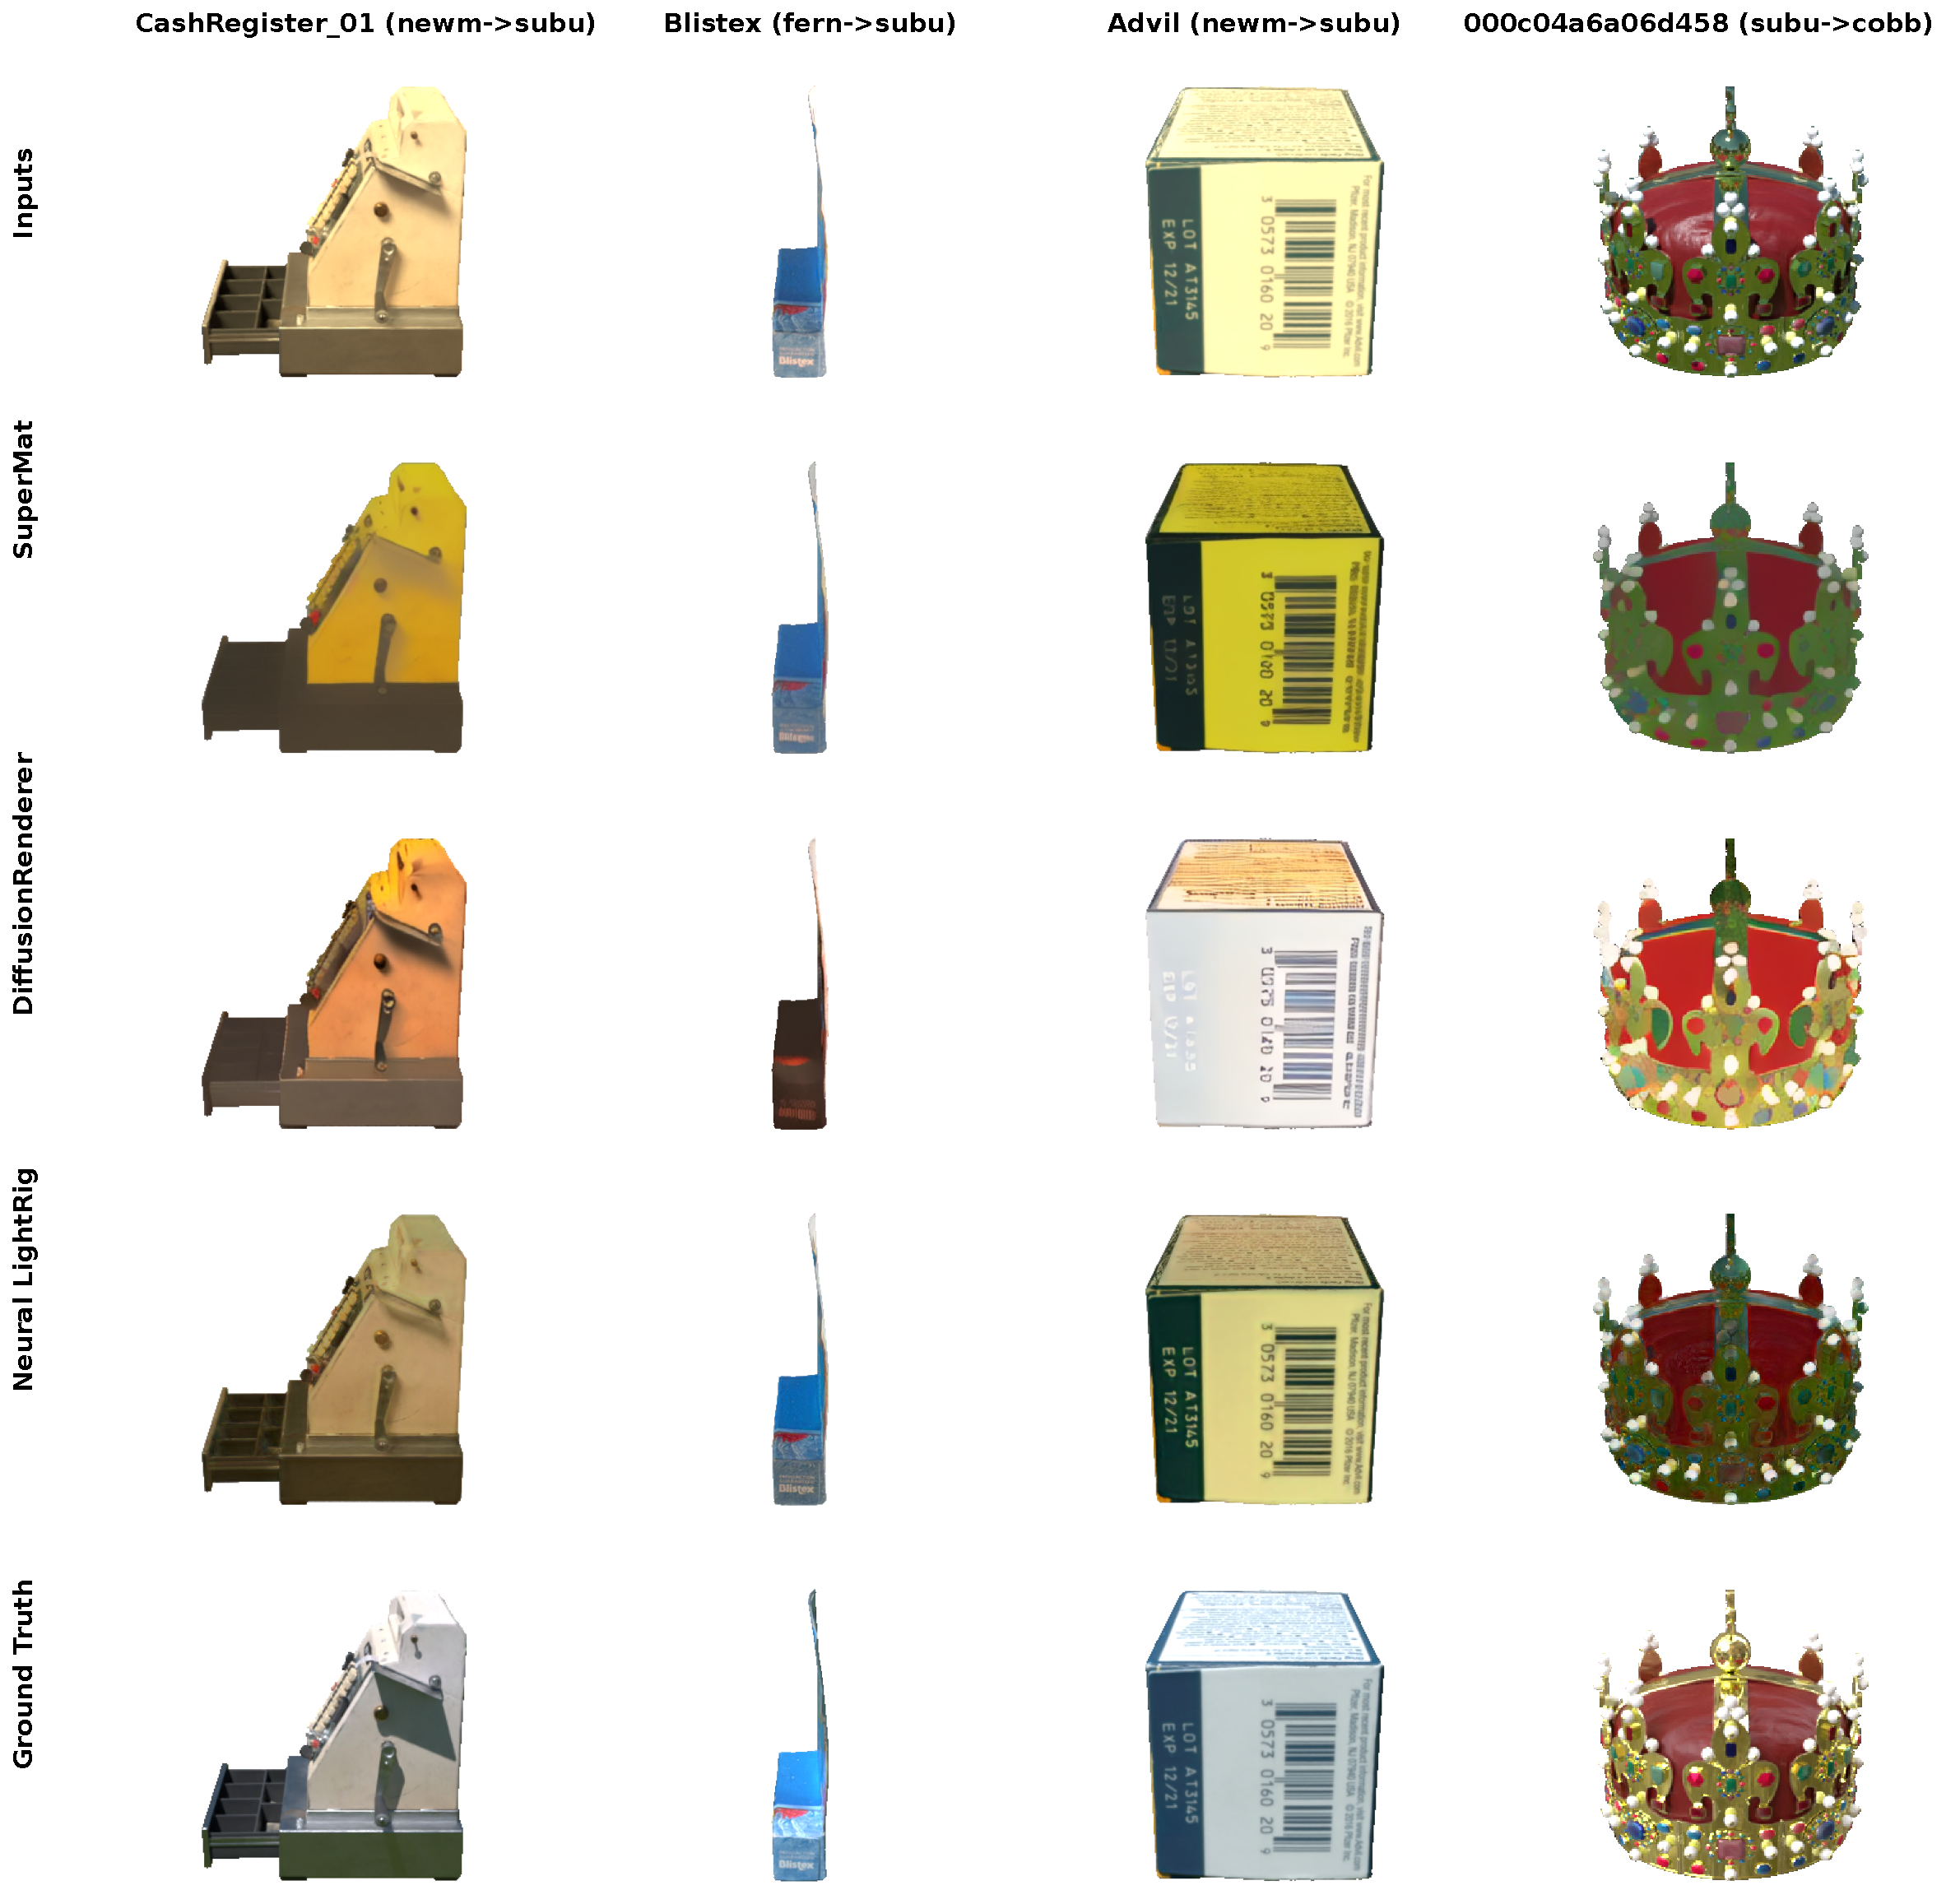
\includegraphics[width=\linewidth]{assets/update_23_07/visuals_rerendering_hard.pdf}
  \caption{\textbf{Indirect relighting evaluation — Hard / Failure Split.} Novel illumination rerender outputs for challenging failure cases.}
  \label{fig:visuals-rerendering-hard}
\end{figure}

\clearpage
\section{Immediate Next Steps}

\begin{enumerate}
  \item Complete full multi-view / 3D-native baseline evaluations (including \textbf{Material Anything}~\cite{materialanything}, \textbf{TRELLIS.2}~\cite{trellis2}, and \textbf{Hunyuan3D 2.1}~\cite{hunyuan3d21}) across all datasets.
  \item Incorporate real-world scanned object splits (e.g. Stanford-ORB / Objects With Lighting).
\end{enumerate}

\section*{References}
\addcontentsline{toc}{section}{References}

\begin{thebibliography}{99}
  \bibitem{neurallightrig}
  Zexin He, Tengfei Wang, Xin Huang, Xingang Pan, and Ziwei Liu.
  \newblock Neural LightRig: Unlocking Accurate Object Normal and Material Estimation with Multi-Light Diffusion.
  \newblock In \emph{CVPR}, 2025.
  \newblock \href{https://arxiv.org/abs/2412.09593}{arXiv:2412.09593}.

  \bibitem{supermat}
  SuperMat: Physically Consistent PBR Material Estimation at Interactive Rates.
  \newblock \emph{arXiv preprint arXiv:2411.17515}, 2024.
  \newblock \href{https://arxiv.org/abs/2411.17515}{arXiv:2411.17515}.

  \bibitem{matmart}
  Xiuchao Wu, Pengfei Zhu, et al.
  \newblock MatMart: Material Reconstruction of 3D Objects via Diffusion.
  \newblock In \emph{CVPR}, 2026.
  \newblock \href{https://arxiv.org/abs/2511.18900}{arXiv:2511.18900}.

  \bibitem{diffusionrenderer}
  DiffusionRenderer: Neural Inverse and Forward Rendering with Video Diffusion Models.
  \newblock In \emph{CVPR}, 2025.
  \newblock \href{https://arxiv.org/abs/2501.18590}{arXiv:2501.18590}.

  \bibitem{materialanything}
  Xin Huang, Tengfei Wang, Ziwei Liu, and Qing Wang.
  \newblock Material Anything: Generating Materials for Any 3D Object via Diffusion.
  \newblock In \emph{CVPR}, 2025.
  \newblock \href{https://arxiv.org/abs/2411.15138}{arXiv:2411.15138}.

  \bibitem{trellis2}
  Native and Compact Structured Latents for 3D Generation (TRELLIS.2).
  \newblock \emph{arXiv preprint arXiv:2512.14692}, 2025.
  \newblock \href{https://arxiv.org/abs/2512.14692}{arXiv:2512.14692}.

  \bibitem{switchlight}
  Hoon Kim, Minje Jang, Wonjun Yoon, Jisoo Lee, Donghyun Na, and Sanghyun Woo.
  \newblock SwitchLight: Co-design of Physics-driven Architecture and Pre-training Framework for Human Portrait Relighting.
  \newblock In \emph{CVPR}, 2024.
  \newblock \href{https://arxiv.org/abs/2402.18848}{arXiv:2402.18848}.

  \bibitem{hunyuan3d21}
  Hunyuan3D 2.1: From Images to High-Fidelity 3D Assets with Production-Ready PBR Material.
  \newblock \emph{arXiv preprint arXiv:2506.15442}, 2025.
  \newblock \href{https://arxiv.org/abs/2506.15442}{arXiv:2506.15442}.

  \bibitem{objaverse}
  Matt Deitke, Dustin Schwenk, Jordi Salvador, Luca Weihs, Oscar Michel, Eli VanderBilt, Ludwig Schmidt, Kiana Ehsani, Aniruddha Kembhavi, and Ali Farhadi.
  \newblock Objaverse: A Universe of Annotated 3D Objects.
  \newblock In \emph{CVPR}, 2023.
  \newblock \href{https://arxiv.org/abs/2212.08051}{arXiv:2212.08051}.

  \bibitem{polyhaven}
  Poly Haven.
  \newblock Poly Haven: The Public 3D Asset Library.
  \newblock \href{https://polyhaven.com}{https://polyhaven.com}, 2024.

  \bibitem{dtc}
  Project Aria.
  \newblock Digital Twin Catalog (DTC) Dataset.
  \newblock \href{https://www.projectaria.com/datasets/dtc/}{Project Aria Datasets}, 2024.

  \bibitem{texverse}
  TexVerse: A Universe of 3D Objects with High-Resolution Textures.
  \newblock \emph{arXiv preprint arXiv:2508.10868}, 2025.
  \newblock \href{https://arxiv.org/abs/2508.10868}{arXiv:2508.10868}.
\end{thebibliography}

\end{document}
